\documentclass{tstextbook}

% for clickable links
%\usepackage{hyperref}

% for longtable (multiple pages)
\usepackage{longtable}

% for 256bit ascii font encoding
\usepackage[T1]{fontenc}

% for lowercase roman enumerations
\usepackage{enumerate}

% define colors
\usepackage{xcolor}
\definecolor{mygreen}{rgb}{0,0.6,0}
\definecolor{mygray}{rgb}{0.5,0.5,0.5}
\definecolor{mymauve}{rgb}{0.58,0,0.82}
\definecolor{darkblue}{rgb}{0.0, 0.0, 0.55}

% languages listings
\usepackage{listings}

% for greek in listings
\usepackage{textgreek}
\lstset{
  literate={ε}{{\textepsilon}}1
}

% listing styles
\lstdefinestyle{Pseudomath}
{
  basicstyle=\ttfamily,
  mathescape
}

\lstdefinestyle{Bash}
{
  language=bash,
  showstringspaces=false,
  %numbers=left,
  %numberstyle=\color{mygray}\textit,
  basicstyle=\footnotesize\ttfamily,
  %keywordstyle=\color{mygreen},
  %commentstyle=\color{mymauve},
  %identifierstyle=\color{blue},
  %stringstyle=\color{orange}
}

\lstdefinestyle{Python}
{
  language=Python,
  showstringspaces=false,
  numbers=left,
  numberstyle=\color{mygray}\textit,
  basicstyle=\footnotesize\ttfamily,
  keywordstyle=\color{mygreen},
  commentstyle=\color{mymauve},
  identifierstyle=\color{blue},
  stringstyle=\color{orange}
}




\begin{document}

\tsbook{Bitcoin Programming}
       {Konstantinos Karasavvas}
       {}
       {2020}
       {}{}{}
       {Version 0.1}
       {}
%       {Cover Designer}
%       {2017}
%       {xxxxx}{xxx--xx--xxxx--xx--x}{0.0}
%       {Publisher}
%       {City}

% Conventions
%---------------------------------------------------------------------------
% using emphbox to emphasize some text or a formula
% using note to NOTE something important
%---------------------------------------------------------------------------

%---------------------------------------------------------------------------
% Chapters
%---------------------------------------------------------------------------

% introduction
% to not include in ToC
%\section*{Preface}

\section{Preface}
This book is not about introducting what Bitcoin is. The readers are expected to understand the basics of the peer-to-peer network, what addresses and private keys are as well as have some experience using wallets and sending bitcoins\footnote{When we refer to the coins we will use \emph{bitcoin(s)} (lowercase `b') and when we refer to the protocol or the network we will use \emph{Bitcoin} (uppercase `B')}. The aim of this book is to help people delve deeper and in particular learn how to \emph{talk} to the Bitcoin network programmatically.

I started teaching Bitcoin programming in 2016. I have given hundreds of presentations in meetups or seminars and from 2017 higher education courses. Every year I was improving and updating my material to keep it as relevant as possible. Luckily, Bitcoin progresses at a steady pace while always keeping backwards compatibility. This is convenient because existing material will always be valid even though better alternatives might be introduced in the future.
  
To understand the material better myself and to improve the material in my courses I started an open source Python library, called bitcoin-utils\footnote{https://github.com/karask/python-bitcoin-utils}. The library was created for educational purposes and not for computational efficiency and that might be evident in certain parts of the implementation. Before starting this library I had investigated several other well-known Python libraries but I did not find an appropriate one for educational purposes. Some were too low-level with limited documentation while others where abstracting concepts that I deemed where important for students to understand.

This book is about teaching Bitcoin programming. Throughout the years I have prepared a lot of material based on my early code experiments, the bitcoin-utils library and several online resources, especially the Bitcoin Stack Exchange\footnote{https://bitcoin.stackexchange.com/} and the excellent Bitcoin Book\footnote{https://github.com/bitcoinbook/bitcoinbook} by A. Antonopoulos. While I try to always credit the initial sources that I have consulted over the years it is very possible that I have missed some. Please let me know and I will update accordingly.

My hope is that this book consolidates all this teaching material with practical examples so as to help others understand Bitcoin programming. 

I have been using a Linux-based machine and thus most command-line examples are from \pyth{bash} shell. However, people comfortable with other Operating Systems should have no issues to adjust as needed.

\chapter{How Bitcoin Works}
\label{ch:howbitcoinworks}

\begin{summary}
This chapter provides a high-level introduction of how Bitcoin works. It aims to be a summary of the prerequisite knowledge required by the reader before moving into the following chapters. The operation of the Bitcoin network is demonstrated with a walkthrough of a transaction and its journey from its creation up until its final destination, the Bitcoin blockchain.
\end{summary}

\section{The Story of a Transaction}
Transactions specify the transfer of bitcoin ownership. Assume we have three actors; Zed, Alice and Bob. Zed has sent 1.5 bitcoins to Alice with $TX_x$ and Alice wants to send 1 bitcoin to Bob. The transaction history will already have an entry of how Alice got her bitcoins (e.g. from Zed).

\begin{note}
Internally, the Bitcoin protocol operates with satoshis: $1~satoshi = 0.00000001~BTC$. Thus, when we want to transfer 1 BTC we actually transfer $100000000~satoshis$.
\end{note}

To send 1 bitcoin (or \emph{BTC}) Alice needs to create a transaction $TX_y$ that sends 1 BTC to Bob. We know that Alice has at least 1.5 BTC from $TX_x$.

\begin{emphbox}
\begin{lstlisting}[style=Pseudomath]
    $TX_x$: 1Zed transfers 1.5 BTC to 1Alice
    $TX_y$: 1Alice transfers 1 BTC to 1Bob
\end{lstlisting}
\end{emphbox}

The names 1Zed, 1Alice and 1Bob are short for the actual bitcoin addresses of Zed, Alice and Bob respectively. So Alice will send 1 BTC from her 1Alice bitcoin address to Bob to his 1Bob address.

Alice has to prove that she is indeed the owner of the address 1Alice when she creates the $TX_y$. Bob does not need to do anything to receive the bitcoins.

A transaction can consist of several \emph{inputs} (outputs of past transactions) and several \emph{outputs} (addresses to send bitcoins to). When an input is used it is completely consumed; i.e. all the bitcoins that the TX contains as inputs need to be \emph{spent}.

\begin{figure}[h]
\begin{center}
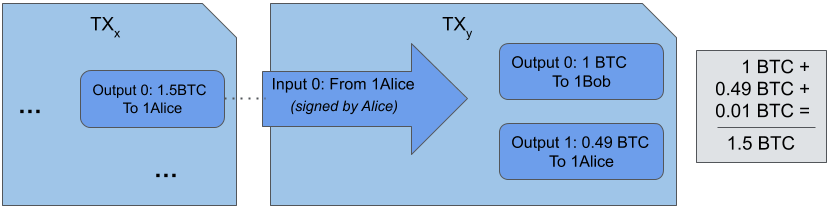
\includegraphics[scale=0.5]{images/typical-transaction}
\caption{Typical one input two outputs transaction.}
\label{fig:typical-transaction}
\end{center}
\end{figure}

The amount of all the inputs needs to be greater or equal to the amounts of outputs. If greater (recommended) the difference is an implied transaction fee that goes to the miners (see figure~\ref{fig:typical-transaction} where the miner receives 0.01 BTC). A typical transaction transfers some bitcoins to another user and returns the remaining bitcoins as change to the originating address or another address that the sender controls.

\begin{note}
For privacy reasons it is recommended to send the change to a different address than the originating. Most bitcoin wallets already do this behind the scenes.
\end{note}

Any number of inputs and outputs is possible as long as a transaction fee is included; the larger the transaction the larger the transaction fee. The unspent outputs are called \emph{Unspent Transaction Outputs (UTXOs)} and the set of UTXOs is essentially all the available bitcoins in the network.

Once a transaction is created it needs to be sent to a Bitcoin node. After the node receives the transaction it checks if it is valid, e.g. the output amounts should be less or equal to the input amounts, the signature proving ownership should be valid, etc. If it is valid the node will propagate it to all its peers\footnote{To be more precise they will notify their peers of the transaction by its \emph{transaction identifier (txid)} and the peers can choose to request it or not. More details will be provided in the Peer-to-Peer chapter.}, i.e. the other nodes that it is aware of. In turn, the other nodes will check if the transaction is valid and so on and so forth until all nodes receive the transaction (see figure~\ref{fig:transaction-propagation}).

\begin{figure}[h]
\begin{center}
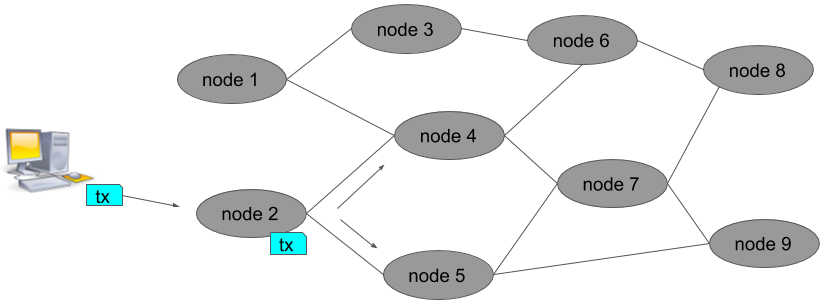
\includegraphics[scale=0.5]{images/transaction-propagation}
\caption{Example of transaction propagation through the network.}
\label{fig:transaction-propagation}
\end{center}
\end{figure}


\section{From Transactions to Blocks}
From a Bitcoin's node perspective, the node receives transactions and places all valid ones into its memory pool, or \emph{mempool}. It keeps receiving new ones until it decides that it will group some of those transactions into a block (see figure~\ref{fig:node-perspective}).

\begin{figure}[h]
\begin{center}
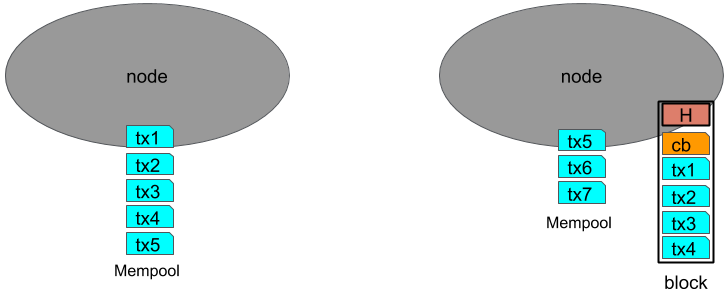
\includegraphics[scale=0.5]{images/node-perspective}
\caption{A node receives transactions into its mempool and can attempt to create new blocks for the network.}
\label{fig:node-perspective}
\end{center}
\end{figure}

%\vspace{3em}
\begin{note}
We are describing what mining nodes typically do. The majority of nodes are not mining nodes and thus do not attempt to create new blocks, rather they validate and propagate valid transactions and blocks when they are aware of them.
\end{note}

Every block contains a \emph{coinbase} transaction that is added by the miner (see next section) and it sends a deterministically calculated reward to an address of the miner's choosing. Finally a header is added to the block containing important information that links this block to its parent and other information that we will examine in the next section.

\section{Mining: basics}
After a node creates a block it will attempt to make it final by propagating it to all other nodes in the network. Multiple nodes will receive the same transactions and will create blocks; nodes choose which TXs to include (see figure~\ref{fig:different-nodes-mining}). They can create and propagate a block at any time.

\begin{emphbox}
But how do we select which blocks will be part of the blockchain? Since, miners include a reward for themselves everyone wants their block to be the next block in the blockchain. In other words, how do we avoid spam and Denial of Service (DoS) attacks?
\end{emphbox}

For a block to be considered valid a miner has to prove that he has done some intensive computational work. Thus, miners have to spend resources before they create a block. This mechanism of proving computational work is called \emph{Proof-of-Work (PoW)} and it involves solving a problem or puzzle. PoW puzzles have the fundamental property of being difficult to solve but trivial to validate their correctness. 

Bitcoin mining is the process of solving the PoW puzzle and selecting the next valid block in a way that is undisputed and thus achieve consensus on the current blockchain state. Bitcoin uses the Hashcash PoW algorithm~\cite{Back2002-hashcash} for its mining.

\begin{figure}[h]
\begin{center}
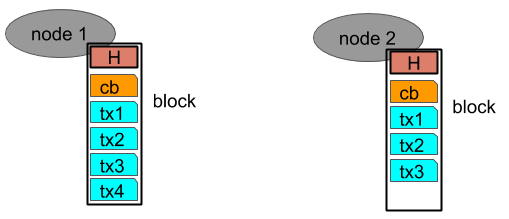
\includegraphics[scale=0.5]{images/different-nodes-mining}
\caption{All nodes will eventually receive all transactions but they are free to include them into a block as they see fit.}
\label{fig:different-nodes-mining}
\end{center}
\end{figure}

The Proof-of-Work puzzle is to compute a cryptographic hash (effectively a big hexadecimal number) of the new block that we want to create which should be less than a target number. The target number that the hash needs to be less than can be deterministically calculated by all nodes and is such that it would take around 10 minutes to calculate with the current network processing power, also called hashing power. Since a hash is random it will take several attempts to find a proper hash but other nodes will verify with only one attempt.

\begin{note}
A cryptographic hash function is a hash function that takes an arbitrary block of data and returns a fixed-size bit string, the cryptographic hash value, such that any (accidental or intentional) change to the data will also change the hash value significantly.
\end{note}

As more miners join the blocks will be created faster so the puzzle’s difficulty automatically adjusts (increases) so that it again requires approximately 10 minutes to solve. This \emph{difficulty adjustment} is happening every 2016 blocks, which is approximately 2 weeks if each block takes 10 minutes to mine.

The hash algorithm used is \keyword{SHA256} and it is applied twice to the block header. As we will see later the header uniquely represents the whole block including all the transactions and thus hashing the header is effectively the same as hashing the whole block, but much more efficiently since the header is much smaller.

\begin{emphbox}
\begin{lstlisting}[style=Pseudomath]
SHA256( SHA256( block_header ) )
\end{lstlisting}
\end{emphbox}

The miner that successfully creates a valid block first will get the bitcoin reward that they have set themselves in the coinbase transaction as well as the fees from all the transactions in the block.

The block reward can be deterministally calculated according to the current \emph{block height}. The reward started at 50 bitcoins and is halved every 210000 blocks (approximately 4 years for 10 minute blocks). So, after block 630000 the reward will be 6.25 bitcoins. The mining reward can be claimed by the miner only after 100 \emph{confirmations}, i.e. after 100 blocks have been confirmed as part of the blockchain since.


\section{Mining: a bit more technical}
\label{sec:mining-technical}

The structure of the block header is as follows:

\begin{center}
\begin{tabular}{ |l|l|l| }
\hline
	Field & Description & Size (bytes)\\
\hline
	version        & Block version number                               & 4\\
	hashPrevBlock  & 256-bit hash of the previous block                 & 32\\
	hashMerkleRoot & 256-bit hash representing all the TXs in the block & 32\\
	timestamp      & Seconds since 1970-01-01T00:00 UTC                 & 4\\
	target (bits)  & The target that the hash should be less than       & 4\\
	nonce          & 32-bit number                                      & 4\\
\hline
\end{tabular}
\end{center}

Block version and timestamp are self explanatory but we will briefly go through the remaining fields.

\subsection*{hashMerkleRoot}
A block has two parts, the header and the transactions. Since we only hash the block header to link blocks together, a header needs to represent the whole block, including all its transactions (coinbase and normal). The transactions are indirectly hashed via using a merkle root and being included in the block by \keyword{hashMerkleRoot}.

A merkle tree\footnote{https://en.wikipedia.org/wiki/Merkle\_tree} is constructed by concatenating all the transaction hashes, in pairs. The resulting hashes are again concatenated and hashed until only a single hash remains, the merkle root.

\begin{figure}[h]
\begin{center}
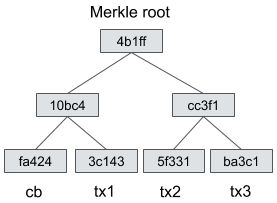
\includegraphics[scale=0.5]{images/merkle-tree}
\caption{Simple merkle root calculation of coinbase and three transactions.}
\label{fig:merkle-tree}
\end{center}
\end{figure}

An important property of a merkle tree is that you can efficiently prove that a hash (and thus transaction) is part of the merkle root. A merkle proof consists of the hashes required to reconstruct the merkle root from the leaf TX, thus proving that the TX hash is indeed part of the merkle tree. For example to prove that \keyword{tx1} is part of the merkle root we would need to provide the hash of \keyword{cb} and its positioning (i.e. left) as well as the parent hash of \keyword{tx2} and \keyword{tx3} (\keyword{cc3f1}) and its positioning (i.e. right).

\subsection*{hashPrevBlock}
This is the hash of the previous block in the blockchain. It designates the parent of the current block and it is effectively what chains the blocks together. For example, if someone changes a transaction in the previous block then the \keyword{hashPrevBlock} will change. This is of particular importance as we will see in more detail in section~\ref{sec:blocks-nakamote-consensus}.

\subsection*{target}
Target bits or just bits is represented as an 8 hex-digit number. The first 2 digits are the exponent and the rest the coefficient. Target bits can be used to calculate the actual target with the following formula:

\begin{emphbox}
\begin{lstlisting}[style=Pseudomath]
    $target = coefficient * 2^{(8 * (exponent - 3))}$
\end{lstlisting}
\end{emphbox}

The highest possible target (the easiest target) is defined as \keyword{0x1d00ffff} and gives a 32-byte target of (expressed as a 64 hexadecimal number):

\small
\begin{emphbox}
\begin{lstlisting}[style=Pseudomath]
0x00000000ffff0000000000000000000000000000000000000000000000000000
\end{lstlisting}
\end{emphbox}
\normalsize

In Python that would be calculated as follows:
\vspace{1em}
\begin{lstlisting}[style=Python,label={lst:encodings-1},caption={Python examples},captionpos=b]
>>> 0x00ffff * 2**(8*(0x1d - 3))
26959535291011309493156476344723991336010898738574164086137773096960
>>> format(26959535291011309493156476344723991336010898738574164086137773096960, '064X')
'00000000FFFF0000000000000000000000000000000000000000000000000000'
\end{lstlisting}
\vspace{1em}



If the result of hashing the block header produces a hash that begins with 0x00000000e (or less) then we have found a solution. That would require, statistically ~$2^{32}$ (4,294,967,296) attempts on average. The smaller the target the more difficult the solution, the more attempts on average.

Another representation of target, easier for humans to understand, is \emph{difficulty} which represents the ratio between the highest target and the current target:

\begin{emphbox}
\begin{lstlisting}[style=Pseudomath]
$Difficulty = \dfrac{highest\_target} {current\_target}$
\end{lstlisting}
\end{emphbox}

When Bitcoin started it started with the highest target (\keyword{0x1d00fff}) and thus it had difficulty 1. Difficulty 1 requires $2^{32}$ attempts on average to find a solution. Difficulty 10 requires $2^{32} * 10$ attempts on average, etc.

\subsection*{nonce}
The nonce is just a number used to differentiate the hash while trying to reach the target. Given that it is only 4 bytes it can only handle ~4.2 billion combinations, while we need quintillion nowadays\footnote{As of August 2020.}.

When the limit was reached miners started modifying the timestamp (e.g. -1 sec) to allow for an additional of ~4.2 billion combinations. However, there is a limit of seconds that a node can deviate from the rest of the network so that did not suffice either\footnote{The timestamp must be higher than the median of the 11 immediate ancestors of the block and higher than the timestamp of its parent. Finally, the timestamp must be no more than 2 hours in the future.}.

Finally, miners started to use the unused space of coinbase's transaction input as an extra nonce allowing an immense amount of extra nonces to be used\footnote{The size of the coinbase input can be from 2 to 100 bytes.}. 


\subsection*{Difficulty Adjustment}
We already mentioned that the difficulty to find the proper hash is expected to take approximately 10 minutes. However, Bitcoin is an open system and anyone can join (or leave) the network as a miner. Thus, the network’s hashrate can increase (or decrease) with time. 

With more hashing power blocks will be issued faster than 10 minutes and thus the network has to adjust the difficulty of the problem accordingly. This can be seen in figure~\ref{fig:hashrate-difficulty}.

\begin{figure}[h]
\begin{center}
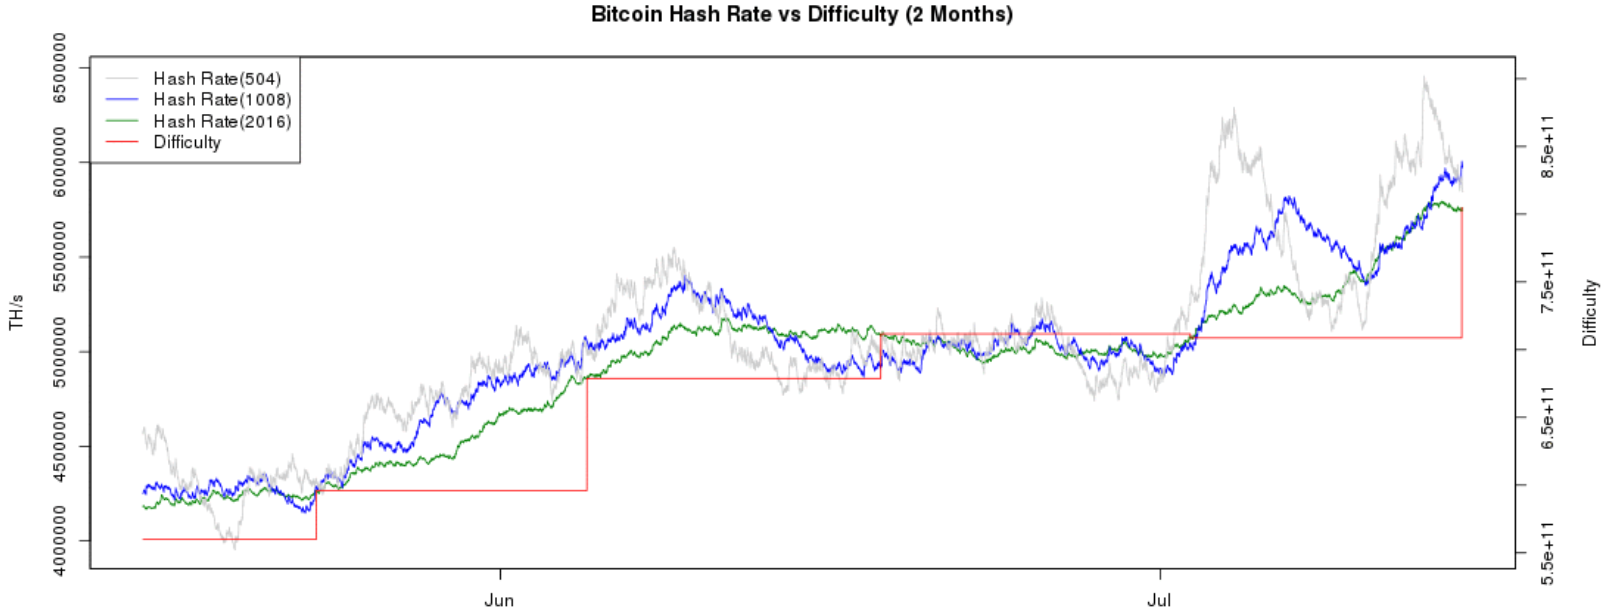
\includegraphics[scale=0.25]{images/hashrate-difficulty}
\caption{Hashrate and difficulty adjustment.}
\label{fig:hashrate-difficulty}
\end{center}
\end{figure}

Specifically, Bitcoin nodes, check every 2016 blocks ($\sim$2 weeks) the timestamps between consecutive blocks and sums them to find out how much time $t$ it took. We want $t$ to take two weeks and thus the new difficulty will be:

\begin{emphbox}
\begin{lstlisting}[style=Pseudomath]
$old\_difficulty * ( \frac{2\_weeks} {t} )$
\end{lstlisting}
\end{emphbox}

\subsection*{Mining Process in a nutshell}
Here we describe a mining node's actions for mining in a simplified step by step process:

\begin{enumerate}
\item Gather valid TXs into blocks
\item Get the longest chain’s top block hash and add it in hashPrevBlock
\item Add timestamp, nonce and extra nonce in the first TX (coinbase)
\item Calculate the merkle root of valid TXs and add it to hashMerkleRoot
\item Hash the header to find a solution smaller than the specified target
  \begin{itemize}
  \item modify timestamp, nonce or extra nonce as appropriate
  \item rehash until a solution is found or the longest chain changed
  \end{itemize}
\end{enumerate}

During the above process:
\begin{itemize}
\item If more TXs are included in the block or the extra nonce is modified
  \begin{itemize}
  \item recalculate merkle root and update it
  \end{itemize}
\item If the longest chain changed we want to build on that chain from now on
  \begin{itemize}
  \item update the valid TX set
  \item update the timestamp
  \item recalculate the merkle root
  \item use the new block as hashPrevBlock
  \end{itemize}
\end{itemize}


\section{The story of a Block}
\label{sec:blocks-nakamote-consensus}
Once a node finds a solution to the PoW problem it will propagate it to its peers. They will check if the block (and every transaction) is valid and if it is they will propagate it to all their peers\footnote{To be more precise they will notify their peers of the block and the peers can choose to request the actual block or not. More details will be provided in the Peer-to-Peer chapter.}. In turn, the peers will check again for the solution as well as the block validity and they will propagate again and so on and so forth until all nodes receive the new block (see figure~\ref{fig:block-propagation}).

\begin{figure}[h]
\begin{center}
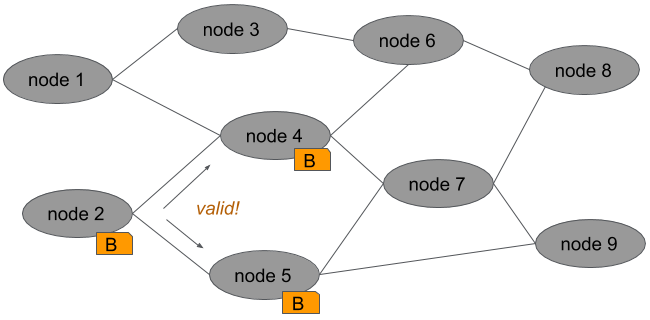
\includegraphics[scale=0.5]{images/block-propagation}
\caption{Example of block propagation through the network.}
\label{fig:block-propagation}
\end{center}
\end{figure}

The new block is being added on top of the existing blocks (every ~10 minutes). This occurs on every single node on the network thus the blocks are the same in all nodes. Blocks are linked with cryptographic hashes forming a chain of blocks, called \emph{Blockchain}.

When Block \keyword{B1} is accepted by the network we say that a transaction on that block has one confirmation. When \keyword{B3} is accepted we say that our transaction has 3 confirmations (see figure~\ref{fig:node-perspective-2}. The more confirmations the more final and secure a transaction is. 

\begin{figure}[h]
\begin{center}
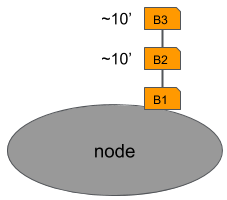
\includegraphics[scale=0.5]{images/node-perspective-2}
\caption{A node receives blocks and links them to form the blockchain.}
\label{fig:node-perspective-2}
\end{center}
\end{figure}


\section{Nakamoto Consensus and Trust}
Each node receives blocks and builds its own blockchain in isolation. A fundamental innovation that bitcoin introduced is the Nakamoto consensus, i.e. how do different nodes come to agreement on what is the current state of the blockchain.

If two miners find a block (almost) at the same time then network peers will get a different block first. They will then start building the next block based on the one they received first. That means that the network at that time has two possible states.

In Nakamoto consensus the basic rule is that miners should \emph{follow the longer chain} (the one with the most computation). Thus, when one of the miners finds the next block all miners will choose the longer chain and consensus is achieved. For an example see the different steps in figure~\ref{fig:nakamoto-consensus}.

\begin{figure}[h]
\begin{center}
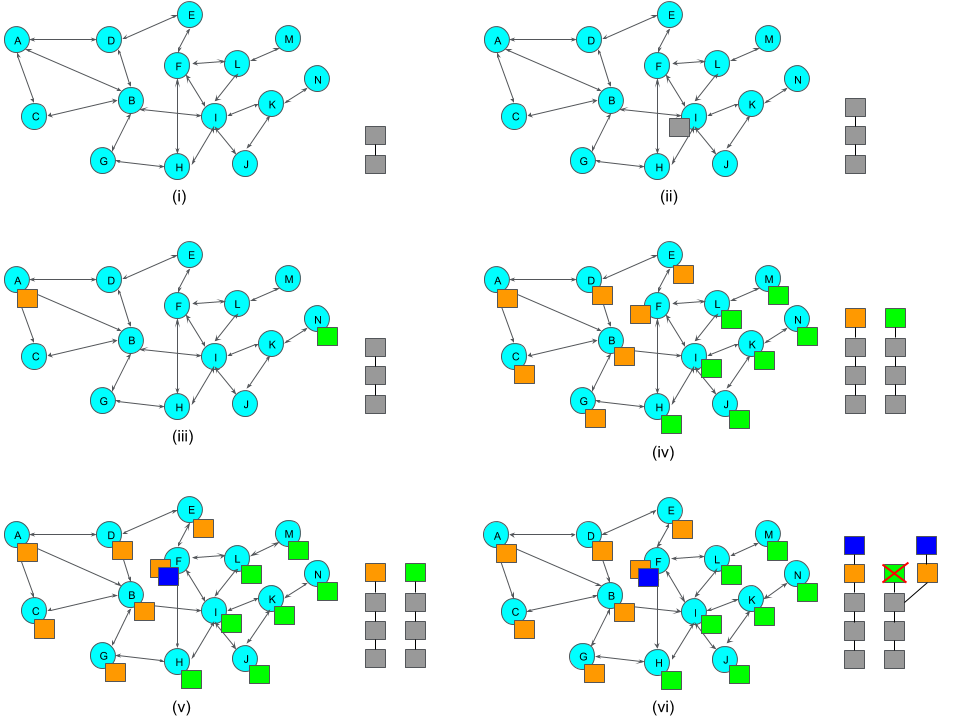
\includegraphics[scale=0.4]{images/nakamoto-consensus}
\caption{Nakamoto Consensus example.}
\label{fig:nakamoto-consensus}
\end{center}
\end{figure}

\begin{enumerate}[(i)]
\item Initially our example network has only two blocks and all nodes are in sync.
\item Then node \keyword{I} finds the next block, which is disseminated to all other nodes and again everyone is in sync.
\item Next, let's suppose that two nodes find a solution at about the same time. These blocks will typically be very similar, including almost the same transactions, but will be different.
\item The nodes will propagate their blocks and some peers will get one of the blocks and some the other. The nodes are aware of both blocks but they will use the block that they received first as the next block and will start mining the next block on top of that block. At this stage we do not have consensus since some of the nodes have a blockchain with the orange block at the top and some the green block.
\item However, after a while a new block will be found. In our example, this is node \keyword{F} and it will propagate it throughout the network.
\item Finally, when the block is propagated to the nodes with the green block on top they will realise that there is a longer chain than the one that they are working on. According to nakamoto consensus the nodes will accept the longer chain as the \emph{valid} chain and ignore the green block. The green block is typically called an \emph{orphan} block\footnote{Precise terminology is more complicated as discussed in https://bitcoin.stackexchange.com/questions/5859/what-are-orphaned-and-stale-blocks}. And now all nodes are in sync again. 
\end{enumerate}

\vspace{3em}
\begin{note}
If there are transactions in the orphaned block that are not in the orange or the blue block they are moved to the mempool ready to be included in one of the following blocks.
\end{note}

Of course it would be possible that at step (v) 2 new solutions could again be found one from a node with an orange block on top and another from a green block on top. Similarly, consenus would be achieved with the following block and two blocks would be orphaned. In such a case, we would say that a 2-block \emph{reorg} occurred.

Nakamoto consensus is a natural and expected reorg event that currently occurs less than once per month\footnote{https://bitcoinchain.com/block\_explorer/orphaned} even for 1-block reorgs. The chance of a reorg is proportional with the number of blocks and thus larger reorgs are exceedingly rare.

\subsection*{Establishing Trust}
As we have seen, blocks are linked together by including the hash of the previous block on the new block. For example, in figure~\ref{fig:blockchain-trust} the hash of \keyword{B1} is included in the header of \keyword{B2}.

\begin{figure}[h]
\begin{center}
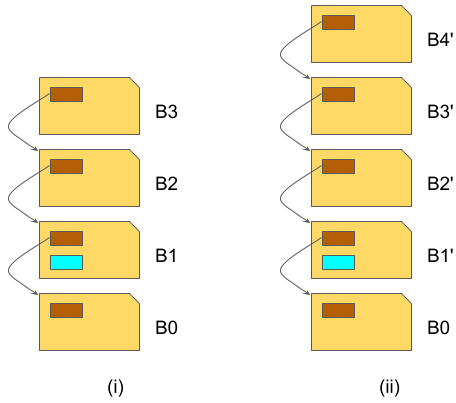
\includegraphics[scale=0.5]{images/blockchain-trust}
\caption{Linked blocks and Trust.}
\label{fig:blockchain-trust}
\end{center}
\end{figure}

In our example a transaction in \keyword{B1} (represented with the cyan box) has 3 confirmations. If an attacker wishes to attempt a double spend attack\footnote{https://en.wikipedia.org/wiki/Double-spending} they will need to create and new \keyword{B1'} block with the modified transaction. However, there are two more blocks on top of \keyword{B1} and thus the attackers block will be ignored since \keyword{B1'} will not be the longer chain. The attacker also needs to create \keyword{B2'}, \keyword{B3'} and \keyword{B4'} to succeed in a double spend. 

To achieve that, the attacker will need to have the majority of the network's hash rate, which is what is typically called the 51\% attack\footnote{Certain attacks, like selfish mining, could be successful with a smaller percentage.}.

Achieving this kind of hash rate and sustaining it would require extravagant amounts of funds to accommodate for the mining hardware and operational costs and thus it would not be easily feasible. 

This is even more evident when one considers what is possible with such an attack: potential censorship and double spends. Even with such an attack the funds on all the Bitcoin addresses are safe as is the historical records of the transactions; the former are secured by strong cryptography while the latter would require much more hash rate to modify them.

Bitcoin security model is based on game theory principles and proper incentives. Economically speaking only a very irrational entity would make such an attack since setting up the environment for the attack would position the attacker in a very economically advantageous position, i.e. they will be earning a lot of money with the mined bitcoins.

\begin{note}
Even though Bitcoin and Nakamoto Consensus provide us with some of the strongest probabilistic guarantees it is theoretically possible to be influenced by malevolent actors. 
\end{note}

Until now the network had been extremely resilient to any kind of attack and has proven its robustness and stability securing hundreds of billions worth of value. The Bitcoin blockchain is considered by many as the most immutable structure constructed by humans.


\section{Basic interaction with a node}
After installing the Bitcoin software\footnote{You can find several online resources on how to install Bitcoin specifically for your operating system. Such tutorial is outside the scope of this book.} we can notice that it includes several executables, one providing the core functionality and the other for interaction and extra utility:
\begin{description}
	\item[bitcoind:] The daemon server that implements the Bitcoin protocol and networking functionality. It also includes a wallet. It provides a JSON-RPC API to talk to the node (ports: mainnet: 8332, testnet: 18332, regtest: 18443, sigtest: 38332).
	\item[bitcoin-cli] Provides a command-line interface to \emph{talk} to the daemon server.
	\item[bitcoin-qt] Provides a graphical user interface to the Bitcoin peer and wallet (subset of the API as part of GUI but also provides a console for all calls).
	\item[bitcoin-tx] Allows to create, parse or modify transactions.
	\item[bitcoin-wallet] Allows to create, parse or modify transactions.
\end{description}

\subsection*{Bitcoin software configuration and development environments}
The configuration file is bitcoin.conf and its default location depends on the operating system used (e.g. in linux system it is located at ~/.bitcoin/bitcoin.conf). Some important options for development and testing\footnote{https://developer.bitcoin.org/examples/testing.html} your application include:

\begin{description}
	\item[deamon=1] Runs the Bitcoin node in the background.
	\item[server=1] Allows JSON-RPC commands but only from localhost.
	\item[testnet=1] The Bitcoin node uses the testnet network for development (i.e. fake funds). If the option is missing or if it is `0' then mainnet (the real network) is used.
	\item[regtest=1] This is a local test environment. The blockchain starts at height 0 (genesis block) and we can trivially mine new blocks with the \keyword{generatetoaddress} command. This allows developers to also control the block creation and get fake funds immediately. Regtest uses testnet’s network parameters (e.g. address prefixes, etc).
	\item[signet=1] New test network for development that adds an additional signature requirement for block validation. Signet is similar in nature to testnet, but more reliable and centrally controlled. Anyone can run their own unique signet for their testing purposes. Available from Bitcoin Core v0.21.0.
	\item[addnode=12.34.56.78] Also connect to specific peer (multiple \keyword{addnode}'s can be used). If no network is specified it will only apply to mainnet.
	\item[connect=12.34.56.78] Only connect to specific node (multiple \keyword{connect}'s can be used). If no network is specified it will only apply to mainnet.
	\item[rpcallowip=12.34.56.78] Allows JSON-RPC connections from this IP (default is localhost).
	\item[prune=1000] Only keep more recent blocks that fit in 1000 MiB. Pruning is not compatible with \keyword{txindex} and \keyword{rescan}. 
	\item[mempoolsize=100] Only keep transactions that fit in 100 MiB. Transactions are ordered by fee rate and if there is not enough space the ones with the lowest fee rate are removed.
\end{description}

We can also include sections like \keyword{main}, \keyword{test} and \keyword{regtest} to provide specific options depending on the network used. Usually, when optioins are not specified under a section they apply to all sections with the exception of \keyword{addnode}, \keyword{connect}, \keyword{port}, \keyword{bind}, \keyword{rpcport}, \keyword{rpcbind} and \keyword{wallet}.

A typical minimalistic config for development is:
\begin{emphbox}
\begin{lstlisting}[style=Bash]
daemon=1
testnet=1
#regtest=1

server=1
rpcuser=kostas
rpcpassword=toodifficulttoguess

[main]
mempoolsize=300

[test]
mempoolsize=100

[regtest]
mempoolsize=20
\end{lstlisting}
\end{emphbox}


\subsection*{Examples of Calls using \keyword{bitcoin-cli}}


To get help of all available commands and how to get further help:
\begin{emphbox}
\begin{lstlisting}[style=Bash]
$ bitcoin-cli help
\end{lstlisting}
\end{emphbox}
\vspace{1em}

After version 0.22 a bitcoin wallet is not created by default. We have to create one ourselves. We can create a default wallet with:

\begin{emphbox}
\begin{lstlisting}[style=Bash]
$ bitcoin-cli -named createwallet wallet_name="testwallet" load_on_startup=true
\end{lstlisting}
\end{emphbox}
\vspace{1em}

\noindent The default wallet is a descriptor wallet (see chapter~\ref{ch:keys-and-addresses} for more on descriptor wallets). To use commands like \keyword{importaddress} and \keyword{dumpprivkey} a non-descriptor wallet needs to be created:

\begin{emphbox}
\begin{lstlisting}[style=Bash]
$ bitcoin-cli -named createwallet wallet_name="testwallet-2" descriptors=false
\end{lstlisting}
\end{emphbox}
\vspace{1em}



\noindent To get the current block height:
\begin{emphbox}
\begin{lstlisting}[style=Bash]
$ bitcoin-cli getblockcount
1806981
\end{lstlisting}
\end{emphbox}
\vspace{1em}

\noindent To get the current balance of all addresses:
\begin{emphbox}
\begin{lstlisting}[style=Bash]
$ bitcoin-cli getbalance
1.51815479
\end{lstlisting}
\end{emphbox}
\vspace{1em}

\noindent To get a new legacy\footnote{The typical P2PKH Addresses starting with \keyword{1} on mainnet and \keyword{m} or \keyword{n} on testnet.} address:
\begin{emphbox}
\begin{lstlisting}[style=Bash]
$ bitcoin-cli getnewaddress "" legacy
mvBGdiYC8jLumpJ142ghePYuY8kecQgeqS
\end{lstlisting}
\end{emphbox}
\noindent By default Bitcoin v0.20+ use \keyword{bech32} (or native segwit) addresses. The example above overrides the default. We will examine the different kind of Bitcoin addresses in Chapter~\ref{ch:keys-and-addresses}.
\vspace{1em}

\noindent To encrypt the wallet with a passphrase:
\begin{emphbox}
\begin{lstlisting}[style=Bash]
$ bitcoin-cli walletencrypt PaSsPhRaSe
wallet encrypted; Bitcoin server stopping, restart to run with encrypted 
wallet. The keypool has been flushed and a new HD seed was generated (if 
you are using HD). You need to make a new backup.
\end{lstlisting}
\end{emphbox}
\vspace{1em}

\noindent To unlock an encrypted wallet for 2 minutes to spend funds:
\begin{emphbox}
\begin{lstlisting}[style=Bash]
$ bitcoin-cli walletpassphrase PaSsPhRaSe 120
\end{lstlisting}
\end{emphbox}
\vspace{1em}

\noindent To create a wallet backup:
\begin{emphbox}
\begin{lstlisting}[style=Bash]
$ bitcoin-cli backupwallet wallet.backup
\end{lstlisting}
\end{emphbox}
\vspace{1em}

\noindent To import a backed up wallet:
\begin{emphbox}
\begin{lstlisting}[style=Bash]
$ bitcoin-cli importwallet wallet.backup
\end{lstlisting}
\end{emphbox}
\vspace{1em}

\noindent To get the node's networking info:
\begin{emphbox}
\begin{lstlisting}[style=Bash]
$ bitcoin-cli getnetworkinfo
{
  "version": 200000,
  "subversion": "/Satoshi:0.20.0/",
  "protocolversion": 70015,
  "localservices": "0000000000000409",
  "localservicesnames": [
    "NETWORK",
    "WITNESS",
    "NETWORK_LIMITED"
  ],
  ... 
}
\end{lstlisting}
\end{emphbox}
\vspace{1em}

\noindent To get the node's blockchain info:
\begin{emphbox}
\begin{lstlisting}[style=Bash]
$ bitcoin-cli getblockchaininfo
{
  "chain": "test",
  "blocks": 1887283,
  "headers": 1887283,
  "Bestblockhash": "0000000000074e...9d44e05b4",
  "difficulty": 1420477.254893854,
  "mediantime": 1604662239,
  "verificationprogress": 0.9999999194957088,
  "initialblockdownload": false,
  "chainwork": "000000000000...a2762e8",
  "size_on_disk": 28640545955,
  "pruned": false,
  ...
}
\end{lstlisting}
\end{emphbox}
\vspace{1em}

\noindent To get the node's mining info:
\begin{emphbox}
\begin{lstlisting}[style=Bash]
$ bitcoin-cli getmininginfo
{
  "blocks": 1887283,
  "difficulty": 1420477.254893854,
  "networkhashps": 131251268159888.9,
  "pooledtx": 9,
  "chain": "test",
  "warnings": "Warning: unknown new rules activated (versionbit 28)"
}
\end{lstlisting}
\end{emphbox}
\vspace{1em}

\noindent To get the node's wallet info:
\begin{emphbox}
\begin{lstlisting}[style=Bash]
$ bitcoin-cli getwalletinfo
{
  "walletname": "wallet-test1",
  "walletversion": 169900,
  "format": "bdb",
  "balance": 0.00065838,
  "unconfirmed_balance": 0.00000000,
  "immature_balance": 0.00000000,
  "txcount": 1,
  "keypoololdest": 1667229693,
  "keypoolsize": 1000,
  "hdseedid": "c41632b90911bb4d4b172190bf9a27def9535fc4",
  "keypoolsize_hd_internal": 1000,
  "paytxfee": 0.00000000,
  "private_keys_enabled": true,
  "avoid_reuse": false,
  "scanning": false,
  "descriptors": false,
  "external_signer": false
}
\end{lstlisting}
\end{emphbox}
\vspace{1em}


\noindent To send 0.01 BTC to address \keyword{mvBGdiYC8jLumpJ142ghePYuY8kecQgeqS} without specifying which UTXOs to use\footnote{You can check the transaction online using a Bitcoin testnet block explorer: https://blockstream.info/testnet/tx/ff8322626c21c5bdfa1d27f75a55a1cb1d3b764bb34063f64b38f0803c370c08}:
\begin{emphbox}
\begin{lstlisting}[style=Bash]
$ bitcoin-cli sendtoaddress mvBGdiYC8jLumpJ142ghePYuY8kecQgeqS 0.01
ff8322626c21c5bdfa1d27f75a55a1cb1d3b764bb34063f64b38f0803c370c08
\end{lstlisting}
\end{emphbox}
\vspace{1em}

\noindent To display all UTXOs with at least 2 confirmations:
\begin{emphbox}
\begin{lstlisting}[style=Bash]
$ bitcoin-cli listunspent 2
[
  {
    "txid": "30d98980c56a139438f0c969ca30d4be2c7f865d098b905362263c5daca2afa7",
    "vout": 0,
    "address": "mgs9DLttzvWFkZ46YLSNKSZbgSNiMNUsdJ",
    "amount": 1.01452015,
    "confirmations": 20183,
    ...
  }
... 
]
\end{lstlisting}
\end{emphbox}
\vspace{1em}

\noindent To check all the available address labels:
\begin{emphbox}
\begin{lstlisting}[style=Bash]
$ bitcoin-cli listlabels
{
  "": 1.01483854,
  ...
}
\end{lstlisting}
\end{emphbox}
\vspace{1em}

\noindent To check all addresses with a particular label:
\begin{emphbox}
\begin{lstlisting}[style=Bash]
$ bitcoin-cli getaddressesbylabel
{ 
  "mvBGdiYC8jLumpJ142ghePYuY8kecQgeqS": {
    "purpose": "receive"
  },
  ...
}
\end{lstlisting}
\end{emphbox}
\vspace{1em}


To get more information for the status of your node you can use commands like: \keyword{getblockchaininfo}, \keyword{getmempoolinfo}, \keyword{gettxoutsetinfo}, \keyword{getmemoryinfo}, \keyword{getrpcinfo}, \keyword{getmininginfo}, \keyword{getnetworkinfo}, \keyword{getpeerinfo}, \keyword{getdescriptorinfo}, \keyword{getaddressinfo}, \keyword{getwalletinfo}.


\section{What to read next?}
We should now have a basic understanding of how Bitcoin works and how to interact with a node. Make sure you are comfortable with the command-line, use \keyword{help} to see what commands are available and experiment!

After that you have some options on how to proceed. If you want some more background knowledge of how the Bitcoin network operates, continue with chapters~\ref{ch:p2p-networking} and~\ref{ch:forking}. If you want to go straight to how to create transactions and write Bitcoin scripts programmatically go directly to chapters~\ref{ch:keys-and-addresses} and ~\ref{ch:scripting-1}. For those who want to go deeper there is also the option to go through the implementation of the \keyword{bitcoin-utils} library. To that end chapter~\ref{ch:technical-fundamentals} will provide some technical knowledge required for understanding the library.



\section{Exercises}

\begin{exercise}
Prepare a bitcoin environment by installing a Bitcoin node configured for testnet. 
\end{exercise}

\begin{exercise}
Using \keyword{bitcoin-cli} create a new legacy address.
\end{exercise}

\begin{exercise}
Use a Bitcoin testnet faucet to get some testnet bitcoins (tBTC) to one of your addresses.
\end{exercise}

\begin{exercise}
Ask your classmates or friends for their testnet address and send them some tBTC using \keyword{bitcoin-cli}.
\end{exercise}

\begin{exercise}
Use a block explorer to see the status of the transaction that you created in the previous exercise.
\end{exercise}

\begin{exercise}
Encrypt your wallet and back it up.
\end{exercise}

\begin{exercise}
Go through the rest of the API and get familiar with more commands.
\end{exercise}

\begin{exercise}
Search for historical data on Bitcoin's difficulty adjustments and make sure you understand what you see.
\end{exercise}



\chapter{Technical Fundamentals}

\begin{summary}
This chapter aims to provide some basic technical computer science background required for later material. It aims to concisely explain some fundamental concepts by providing examples. 
\end{summary}

\section{Bytes, Hex, Endianness and Encodings}
Computers internally use the binary numeral system that consists of only two symbols: 0 and 1. A binary digit, or bit, is the basic unit of binary. Eventually, everything is represented in bits.

For ease of processing, bits are aggregated into bytes. Each byte consists of 8 bits. Thus, \keyword{01000001} represents a single byte. It is difficult (and much longer) to use/type binary, thus we typically use the hexadecimal numeral system or hex to represent bytes in a more human-friendly way. Hex has 16 possible symbols from 0 to F (0-9 and A-F). To represent 16 symbols we need exactly 4 bits (0 is 0000, 1 is 0001, …, F is 1111) and thus each byte can be represented by two hex digits. For example, \keyword{01000001} is equivalent to \keyword{41} in hexadecimal (0100 is hex number 4 and 0001 is hex number 1). You can experiment with conversions between binary, hexadecimal and decimal using various online tools\footnote{https://www.rapidtables.com/convert/number/binary-to-hex.html}.

\vspace{1em}
\begin{lstlisting}[style=Python,label={lst:encodings-1},caption={Python examples},captionpos=b]
>>> format(0, '04b')      # converts decimal 0 to binary with 0 padding for 4 bits
'0000'
>>> format(15, '04b')     # same for decimal 15
'1111'
>>> format(15, 'X')       # convert decimal 15 to hex string
'F'
>>> format(0x41, '08b')   # converts hex number 41 to binary with 0 padding for
                          # 8 bits
'01000001'
>>> 0x41                  # converts hex number 41 to decimal
65
>>> 0x41 == '41'          # compares hex number 41 with string 41
False
>>> b'41' == '41'         # compares byte literal 41 with string 41
False
\end{lstlisting}
\vspace{1em}

One byte can represent up to $2^8=256$ numbers (0-255). Several bytes are needed to represent larger numbers. For example, decimal number 1000 is \keyword{1111101000} in binary which requires 10 bits. Computers operate at the byte level and thus 2 bytes (or 16 bits) will be required to represent this number; binary: \keyword{0000001111101000} and hex: \keyword{03E8}. Note that the byte ordering is important and it is called endianness\footnote{https://en.wikipedia.org/wiki/Endianness}. The above example uses big-endian ordering, where the most significant byte comes first and the least significant byte comes last. This is the same way we order numbers in languages (in left-to-right scripts\footnote{https://en.wikipedia.org/wiki/Writing\_system\#Directionality}). In little-endian the same number would be represented as \keyword{1110100000000011} and \keyword{E803}.

\vspace{1em}
\begin{lstlisting}[style=Python,label={lst:encodings-2},caption={Python examples},captionpos=b]
>>> import binascii
>>> format(0x03E8, '016b')           # convert hex number 03E8 to binary digits
                                     # with 0 padding for 16 bits
'0000001111101000'
>>> format(int('03E8', 16), '016b')  # convert hex string '03E8' to binary digits 
                                     # as above
'0000001111101000'
>>> binascii.unhexlify('03E8')       # convert hex string 03E8 to binary
b'\x03\xe8'
>>> b'\x03\xe8'[::-1]                # reverse bytes to change endianness
b'\xe8\x03'
\end{lstlisting}
\vspace{1em}


\begin{note}
Internally Bitcoin uses little-endian byte order as it improves speed (most computers use little-endian byte ordering internally). Most hash function libraries (see next section) create hashes using big-endian and Bitcoin transmits those in that ordering. However, when hashes are displayed Bitcoin uses little-endian order! The latter might be because it treats them as integers to compare them faster.
\end{note}

As we already mentioned computers only know about binary. To display these numbers for human consumption we need to convert them into characters (i.e. text). In order to accomplish that we need character encodings that provide mappings between bit sequences and characters. Examples of such encodings are ASCII and UTF-8. UTF-8 is widely used nowadays and it provides an 8-bit mapping between (binary) numbers and characters. For example, character \keyword{A} is mapped to \keyword{01000001}. You can experiment with such encodings with online tools\footnote{https://www.rapidtables.com/convert/number/ascii-to-binary.html}.

\vspace{1em}
\begin{lstlisting}[style=Python,label={lst:encodings-3},caption={Python examples},captionpos=b]
>>> import binasci
>>> 'A' == b'A'                      # A character is not a byte
False
>>> b'41' == '41'.encode('utf-8')    # Unicode string literals are stored internally
                                     # in binary for efficiency
True
>>> 'ε'.encode()                     # UTF-8 (the default) is a variable lenth
                                     # encoding - 'ε' is stored as two bytes
b'\xce\xb5'
>>> '41'.encode()                    # converts UTF-8 string literal 41 to binary -
                                     # '4' and '1' occupy 1 byte each
b'41'
>>> binascii.unhexlify('41')         # converts string hex value 41 to binary - 
                                     # the UTF-8 value for 'A' is 0x41
b'A'
>>> b'A' == b'\x41'                  # the bytes from 0x01 to 0x7f are confusingly
                                     # specified with UTF-8 characters
True
>>> b'41' == b'\x34\x31'             # similarly for binary characters b'4' and
                                     # b'1' or b'41'
True
>>> b'A'.decode('utf-8')             # convert binary to characters for displaying
                                     # according to UTF-8 encoding
'A'
>>> binascii.hexlify(b'A')           # convert binary value to hex value (expressed
                                     # in binary)
b'41'
>>> b'41'.decode()                   # decode to get as string (UTF-8 is the default)
'41'
>>> b'\xce\xb5'.decode()             # convert from bytes to UTF-8 characters (0xce
                                     # 0xb5 maps to 'ε')
'ε'
\end{lstlisting}
\vspace{1em}


\section{Cryptographic Hash Functions}
A cryptographic hash function is a hash function that is suitable for cryptography. It is an one-way function that takes an arbitrary block of data and returns a fixed-size bit array, that is called the hash value or digest or digital fingerprint or just hash. It has the following properties:

\begin{itemize}
\item it is deterministic, i.e. the same block of data always returns the same hash
\item it is quick to compute
\item it is an one-way function; given the hash one cannot derive the original value unless they brute-force all possible values (which is close to impossible for large data sets)
\item even a trivial change to the original data will change the resulting hash completely (it will appear uncorrelated to the previous hash)
\item it is collision resistant; it is computational infeasible to find two different blocks of data with the same hash value
\end{itemize}

\vspace{1em}
\begin{lstlisting}[style=Python,label={lst:encodings-4},caption={Python examples},captionpos=b]
>>> import hashlib
>>> import binascii
>>> b1 = 'Bitcoin'.encode('utf-8')   # convert string to bytes according to UTF-8 
                                     # encoding
>>> b1
b'Bitcoin'
>>> h1 = hashlib.sha256(b1).digest() # calculate the hash (or digest) of b1
>>> h1
b'\xb4\x05m\xf6i\x1f\x8d\xc7.V0-\xda\xd3E\xd6_\xea\xd3\xea\xd9)\x96\t\xa8&\xe24N' \
b'\xb6:\xa4'
>>> binascii.hexlify(h1).decode()    # converts bytes to hex (expressed in binary)
                                     # and then to string to display
'b4056df6691f8dc72e56302ddad345d65fead3ead9299609a826e2344eb63aa4'
>>> b2 = 'bitcoin'.encode('utf-8')   # convert string to bytes according to UTF-8
                                     #encoding
>>> b2
b'bitcoin'
>>> h2 = hashlib.sha256(b2).digest() # calculate the hash (or digest) of b2
>>> h2
b'k\x88\xc0\x87$z\xa2\xf0~\xe1\xc5\x95k\x8e\x1a\x9fL\x7f\x89*p\xe3$\xf1\xbb=\x16' \
b'\x1e\x05\xca\x10{'
>>> binascii.hexlify(h2).decode()    # converts bytes to hex (expressed in binary)
                                     # and then to string to display
'6b88c087247aa2f07ee1c5956b8e1a9f4c7f892a70e324f1bb3d161e05ca107b'
\end{lstlisting}
\vspace{1em}

Cryptographic hash functions are very important in information security systems. They are used in digital signatures, message authentication codes and as ordinary (but more secure) hash functions to index data in hash tables, to uniquely identify files (bittorrent, IPFS), as checksums to detect accidental (or not) corruption of data, etc.

\begin{note}
Bitcoin is using two hashing functions: SHA-256 and RIPEMD-160 which create a hash value of 256 and 160 bits respectively (or 32 and 20 bytes or 64 and 40 hex characters).
\end{note}

\section{Asymmetric Cryptography}
Asymmetric cryptography or public key cryptography\footnote{https://en.wikipedia.org/wiki/Public-key\_cryptography} is a cryptographic system that uses pairs of keys with a specific mathematical relation. In each pair there is a private key that should remain private and a public key that can be freely shared. Between two participants this allows:

\begin{itemize}
\item Encryption: Alice can encrypt a message with Bob’s public key and send it to Bob. Only the owner of the corresponding private key can decrypt and view the message.
\item Authentication / Digital Signatures: Alice can sign a message using her private key and send it to Bob. Anyone can view the contents and verify the signature using Alice’s public key, thus ensuring that it was indeed Alice that send the message.
\item Integrity: While anyone can view the contents of a signed message no one can modify it since the signature will be invalidated.
\item Non-Repudiation: Signing or encrypting a message cannot be refuted by the author once the message has been sent, assuming the private key is secure.
\end{itemize}


\begin{note}
Bitcoin does not use encryption at all. Digital signatures are used to sign transactions in order to authenticate that you are the owner of the coins you wish to transfer. Integrity and non-repudiation apply as well to transaction signing.
\end{note}

There are several different algorithms for asymmetric cryptography, like RSA and ECDSA. ECDSA, which Bitcoin uses, has the property that a private key can be used to calculate the corresponding public key.



\chapter{Keys and Addresses}
\label{ch:keys-and-addresses}

\begin{summary}
In this chapter we introduce Bitcoin’s keys and addresses and describe how they are created and the rationale behind that process. We then go through different wallet types and how these keys can be used in practice.
\end{summary}

\section{Private Keys}
Bitcoin uses the Elliptic Curve Digital Signature Algorithm (ECDSA)\footnote{https://en.wikipedia.org/wiki/Elliptic\_Curve\_Digital\_Signature\_Algorithm} to create its private-public key pairs. The exact elliptic curve parameters used in Bitcoin are defined by secp256k1\footnote{https://en.bitcoin.it/wiki/Secp256k1}.

\begin{note}
In ECDSA a private key can be used to calculate the corresponding public key, and since a Bitcoin address is calculated from the public key, if you hold a private key securely you effectively have everything.
\end{note}

The ECDSA private key in Bitcoin is just a very large random number consisting of 256 bits or 32 bytes or 64 hexadecimal digits. Nearly all 256-bit numbers can be valid private keys as specified in secp256k1.

To display a private key (the bytes) we need to format it appropriately. It could be displayed in hex but the most common format used to display a private key is Wallet Import Format (WIF) or WIF-compressed (WIFC); both are a Base58Check\footnote{https://en.bitcoin.it/wiki/Base58Check\_encoding} encoding of the ECDSA key; Base58\footnote{https://en.wikipedia.org/wiki/Base58} with a version prefix to specify the network and a 32-bit checksum.

A WIF-compressed adds an extra byte (0x01) at the end of the ECDSA key before the Base58Check encoding. It specifies whether the public key (and by extension addresses) will be compressed or not. By default most wallets use WIFC format in order to reduce the size of the blockchain\footnote{Note that the segregated witness upgrade allows only compressed public keys.}.


\begin{note}
The WIFC will be 33 bytes long. The compression is happening when creating the public key which will be 33 bytes instead of 65 bytes.
\end{note}

The following is pseudocode of the process that converts the private key to WIF.

\begin{emphbox}
%\begin{lstlisting}[style=Pseudomath,label={lst:wif-pseudocode},caption={Pseudocode to convert a private key to the WIF format},captionpos=b]
\begin{lstlisting}
key_bytes = (32 bytes number) [ + 0x01 if compressed ]
network_prefix = (1 byte version number)
data = network_prefix + key_bytes
data_hash = SHA-256( SHA-256( data ) )
checksum = (first 4 bytes of data_hash)
wif = Base58CheckEncode( data + checksum )
\end{lstlisting}
\end{emphbox}

Note that all the above functions operate on big-endian bytes. The network prefix specifies the Bitcoin network that this private key would be used\footnote{The same private key can be of course used in both mainnet and testnet or even other compatible cryptocurrencies by using the appropriate prefix when generatig the WIF.}. The Base58 WIF prefix depends on the network prefix and whether it is compressed or not, as shown in table~\ref{tab:private-key-prefixes}.

\begin{table}[h]
\centering
\begin{tabular}{ |l|c|c|c|c| }
\hline
~ & \multicolumn{2}{c|}{\textbf{Mainnet}} & \multicolumn{2}{c|}{\textbf{Testnet}} \\
\hline
ECDSA HEX & \multicolumn{2}{c|}{64 digits number} & \multicolumn{2}{c|}{64 digits number} \\
\hline
ECDSA HEX-C & \multicolumn{2}{c|}{Above number + ``01''} & \multicolumn{2}{c|}{Above number + ``01''} \\
\hline
~ & \textbf{Network Prefix} & \textbf{Base58 Prefix} & \textbf{Network Prefix} & \textbf{Base58 Prefix} \\
\hline
WIF & 128 | 0x80 & 5 & 239 | 0xef & 9 \\
\hline
WIF-C & 128 | 0x80 & K or L & 239 | 0xef & c \\
\hline
\end{tabular}
\caption{Private keys network prefixes}
\label{tab:private-key-prefixes}
\end{table}

As an example let us use the following hexadecimal number\footnote{In decimal: 6273083586486421860511804118443655246000698298582245067579657211. It is important to understand that a random number with enough entropy is required for your private key to be secure. A number representing your date of birth or your name’s characters, etc. will be found immediately by software and you will lose your funds.}:

\begin{emphbox}
0dde70823a4bb0ca3bd75a2010e8d5dc091185e73d8b4257a981c695a3eba95b
\end{emphbox}

You can now consult table~\ref{tab:private-key-example} for its compressed version and the corresponding WIF and WIF-C.

\begin{table}[h]
\centering
\begin{tabular}{ |l|l| }
\hline
HEX & 0dde70823a4bb0ca3bd75a2010e8d5dc091185e73d8b4257a981c695a3eba95b \\
\hline
HEX-C & 0dde70823a4bb0ca3bd75a2010e8d5dc091185e73d8b4257a981c695a3eba95b\textbf{01} \\
\hline
WIF & 91h2ReUJRwJhTNd828zhc8RRVMU4krX9q3LNi4nVfiVwkMPfA9p \\
\hline
WIF-C & cN3fHnPVw4h7ZQSRz2HgE3ko69LTaZa5y3JWpFhoXtAke4MiqVQo \\
\hline
\end{tabular}
\caption{Private key network prefix examples}
\label{tab:private-key-example}
\end{table}

Let's use the bitcoin-utils library to construct the WIF and WIFC.

\vspace{1em}
\begin{lstlisting}[style=Python,label={lst:construct-wif},caption={Example of creating WIF and WIFC using Python},captionpos=b]
>>> from bitcoinutils.setup import setup
>>> from bitcoinutils.keys import PrivateKey
>>> setup('testnet')                                   # use testnet parameters
'testnet'
>>> secret_exponent = 0x0dde70823a4bb0ca3bd75a2010e8d5dc091185e73d8b4257a981c695a3eba95b
>>> priv = PrivateKey(secret_exponent = secret_exponent)
>>> priv.to_wif(compressed=False)
'91h2ReUJRwJhTNd828zhc8RRVMU4krX9q3LNi4nVfiVwkMPfA9p'
>>> priv.to_wif(compressed=True)                       # the default
'cN3fHnPVw4h7ZQSRz2HgE3ko69LTaZa5y3JWpFhoXtAke4MiqVQo'
\end{lstlisting}
\vspace{1em}

The actual Python implementation of the functionality demonstrated above can be found at \keyword{to\_wif()}\footnote{\url{https://github.com/karask/python-bitcoin-utils/blob/42875a3fa90d267f2e5e17e017cb28fc8a90c5a8/bitcoinutils/keys.py\#L169-L193}} on github. You can also check how we can get to the private key bytes from WIF in \keyword{\_from\_wif()}\footnote{\url{https://github.com/karask/python-bitcoin-utils/blob/42875a3fa90d267f2e5e17e017cb28fc8a90c5a8/bitcoinutils/keys.py\#L129-L166}}. Feel free to consult the rest of the code and/or the examples in the repository.

Another tool that you can use from the command line is BX\footnote{https://github.com/libbitcoin/libbitcoin-explorer/wiki/Download-BX}. It has extensive capabilities including creating WIFs.

\begin{emphbox}
\begin{lstlisting}[style=Bash]
$ ./bx base58check-encode --version 239 \\
0dde70823a4bb0ca3bd75a2010e8d5dc091185e73d8b4257a981c695a3eba95b
91h2ReUJRwJhTNd828zhc8RRVMU4krX9q3LNi4nVfiVwkMPfA9p

$ ./bx base58check-encode --version 239 \\
0dde70823a4bb0ca3bd75a2010e8d5dc091185e73d8b4257a981c695a3eba95b01
cN3fHnPVw4h7ZQSRz2HgE3ko69LTaZa5y3JWpFhoXtAke4MiqVQo
\end{lstlisting}
\end{emphbox}


\section{Public Keys}
In ECDSA a public key is generated from the private key. Elliptic curves operate over finite fields\footnote{https://en.wikipedia.org/wiki/Finite\_field} and thus all points on the curve are limited to integer coordinates; a finite field is typically accomplished by applying modulo p, where p is a prime number. The specific curve that Bitcoin uses (secp256k1) is  $y^2 = x^3 + 7$ (see figure~\ref{fig:ecdsa-curve}\footnote{From https://cryptobook.nakov.com/asymmetric-key-ciphers/elliptic-curve-cryptography-ecc}). Then the public key P is generated by multiplying, using elliptic curve multiplication, the private key k with a special constant G called the generator point\footnote{This is a special point in the elliptic curve that is pre-defined in secp256k1.}: $P = k * G$. Elliptic curve multiplication of an integer with a point results in another point in the curve, which is the public key.

\begin{figure}[h]
\begin{center}
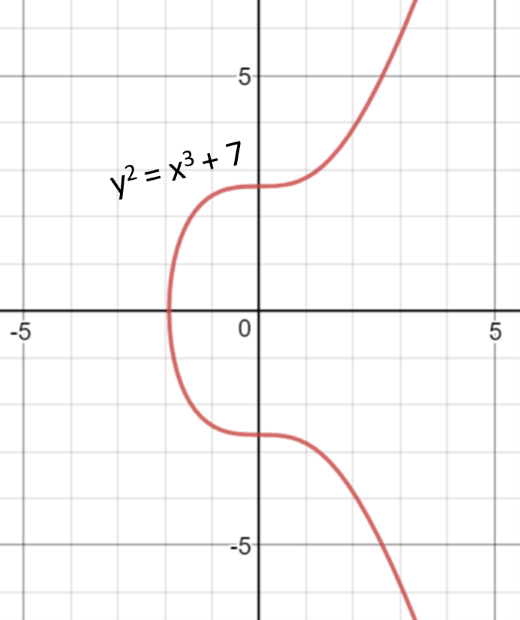
\includegraphics[scale=0.5]{images/ecdsa-curve}
\caption{The secp256k1 ECDSA curve.}
\label{fig:ecdsa-curve}
\end{center}
\end{figure}

The public key is a point $P$ in the elliptic curve. $P = (x,y)$, where both $x$ and $y$ are 32-byte integers. Thus a public key can be expressed with 64 bytes. In Bitcoin, we encode a public key by a prefix that specifies some extra information.

\begin{note}
Remember that we can represent a public key in two forms, compressed and uncompressed. This is where we can reduce the size of the blockchain by using the compressed form.
\end{note}

An encoded uncompressed public key is 65 bytes long since it has the two points (32 bytes each) concatenated and a prefix of \keyword{0x04} to specify an uncompressed public key.

Since the curve is mirrored in the x axis the y coordinate can only take 2 values for a specific x (positive/negative). Thus, an encoded compressed public key is only 33 bytes long and has only the x coordinate with a prefix of \keyword{0x02} (when y is positive/even) or \keyword{0x03} (when y is negative/odd).

Let's use the bitcoin-utils library to construct a private key object from a WIF and use that to create a public key object to show its two forms.

\vspace{1em}
\begin{lstlisting}[style=Python,label={lst:display-public-keys},caption={Example of getting compressed and uncompressed public keys using Python},captionpos=b]
>>> from bitcoinutils.setup import setup
>>> from bitcoinutils.keys import PrivateKey, PublicKey
>>> setup('testnet')
'testnet'
>>> priv = PrivateKey.from_wif('91h2ReUJRwJhTNd828zhc8RRVMU4krX9q3LNi4nVfiVwkMPfA9p')
>>> pub = priv.get_public_key()
>>> pub.to_hex()                # default is compressed form
'02c1acdac799fb0308b4b6475ddf7967676759d31484ab55555482472f3bc7c3e7'
>>> pub.to_hex(compressed=False)
'04c1acdac799fb0308b4b6475ddf7967676759d31484ab55555482472f3bc7c3e7\\
addc4cbba6656a4be4bc6933a6af712b897a543a09c4b899e5f7b943d38108a8'
\end{lstlisting}
\vspace{1em}

You can see in lines 10-11 in listing~\ref{lst:display-public-keys} that the uncompressed public key has the same $x$ coordinate as the compressed one plus the $y$ coordinate.

To create the PublicKey from the PrivateKey object we make use\footnote{It is always recommended to reuse well-tested cryptography libraries than implementing your own.} of the python ecdsa library as can be seen in \keyword{get\_public\_key()} on github\footnote{\url{https://github.com/karask/python-bitcoin-utils/blob/fb0849f81117943563b17f1870a9607d48ca9653/bitcoinutils/keys.py\#L351-L355}}. The PublicKey object holds the $x$ and $y$ coordinates and can convert accordingly. It checks if $y$ is even or odd and prefixes it with $0x02$ and $0x03$ respectively. You can check the code of \keyword{to\_hex()} on github\footnote{\url{https://github.com/karask/python-bitcoin-utils/blob/fb0849f81117943563b17f1870a9607d48ca9653/bitcoinutils/keys.py\#L453-L469}}.

We can get the public keys from the private keys using BX again.

\begin{emphbox}
\begin{lstlisting}[style=Bash]
$ ./bx wif-to-public 91h2ReUJRwJhTNd828zhc8RRVMU4krX9q3LNi4nVfiVwkMPfA9p
04c1acdac799fb0308b4b6475ddf7967676759d31484ab55555482472f3bc7c3e7\\
addc4cbba6656a4be4bc6933a6af712b897a543a09c4b899e5f7b943d38108a8

$ ./bx wif-to-public cN3fHnPVw4h7ZQSRz2HgE3ko69LTaZa5y3JWpFhoXtAke4MiqVQo
02c1acdac799fb0308b4b6475ddf7967676759d31484ab55555482472f3bc7c3e7
\end{lstlisting}
\end{emphbox}


\section{Addresses}
\label{sec:addresses}
Addresses can be shared to anyone who wants to sent you money. They are typically generated from the public key, consist of a sequence of characters and digits and start with 1 for the mainnet and with m or n for testnet\footnote{Or for segwit addresses bc1 and tb1 for mainnet and testnet respectively.}.

An address typically represents the owner of a private/public pair but it can also represent a more complex script as we will see in a future chapter.

Notice that we do not share the public key as one would expect in public key cryptography but rather the address, which derives from the public key. Some benefits are:

\begin{itemize}
\item shorter addresses
\item quantum computer resistance
\end{itemize}

\begin{note}
Until one spends from an address the public key will never appear on the blockchain and thus to potential attackers and since the address is hashed from the public key not even quantum computers could, arguably, brute force to get the public key and then the private key. Note, however, that even if that is the case the majority of addresses would be hacked thus destroying trust in (and the value of) the network anyway!
\end{note}

\subsection*{Legacy Addresses}

An address is really just the hash of the public key, called public key hash (or PKH). That is how it is represented on the blockchain. The way we format addresses to display them (starting with 1, m/n, etc.) are just for our convenience. The format that we use is the Base58Check encoding of the public key hash; Base58 with version prefix to specify the network and a 32-bit checksum.

The following is pseudocode of the process that converts the public key to public key hash and then address:

\begin{emphbox}
%\begin{lstlisting}[style=Pseudomath,label={lst:address-pseudocode},caption={Pseudocode to convert a public key to an address},captionpos=b]
\begin{lstlisting}
network_prefix = (1 byte version number)
keyHash = RIPEMD-160( SHA-256( publicKey ) )
data = network_prefix + keyHash
dataHash = SHA-256( SHA-256( data ) )
checksum = (first 4 bytes of dataHash)
address = Base58CheckEncode( data + checksum )
\end{lstlisting}
\end{emphbox}

Note that all the above functions operate on big-endian bytes. The network prefix specifies the Bitcoin network that this private key would be used. The Base58 WIF prefix depends on the network prefix and whether it is compressed or not, as shown in table~\ref{tab:address-prefixes}.

\begin{table}[h]
\centering
\begin{tabular}{ |l|c|c|c|c| }
\hline
~ & \multicolumn{2}{c|}{\textbf{Mainnet}} & \multicolumn{2}{c|}{\textbf{Testnet}} \\
\hline
~ & \textbf{Network Prefix} & \textbf{Base58 Prefix} & \textbf{Network Prefix} & \textbf{Base58 Prefix} \\
\hline
P2PKH & 0 | 0x00 & 1 & 111 | 0x6f & m or n \\
\hline
P2SH & 5 | 0x05 & 3 & 196 | 0xc4 & 2 \\
\hline
\end{tabular}
\caption{Addresses network prefixes}
\label{tab:address-prefixes}
\end{table}

\keyword{P2PKH} stands for Pay to Public Key Hash and is the typical legacy address. \keyword{P2SH} stands for Pay to Script Hash and is the typical legacy script hash address.

Let's use the bitcoin-utils library to construct some addresses; compressed and uncompressed.

\vspace{1em}
\begin{lstlisting}[style=Python,label={lst:display-addresses},caption={Example of displaying the addresses of compressed and uncompressed public keys using Python},captionpos=b]
>>> from bitcoinutils.setup import setup
>>> from bitcoinutils.keys import PrivateKey, PublicKey, P2pkhAddress
>>> setup('testnet')
'testnet' 
>>> priv = PrivateKey.from_wif('91h2ReUJRwJhTNd828zhc8RRVMU4krX9q3LNi4nVfiVwkMPfA9p')
>>> pub = priv.get_public_key()  
>>> addr1 = pub.get_address()
>>> addr2 = pub.get_address(compressed=False)
>>> addr1.to_string()
'n42m3hGC52QTChUbXq3QAPVU6nWkG9xuWj' 
>>> addr2.to_string() 
'n2JjAgC6UqFf8DvsZXhWcyNzm8w8YKj7MQ'
\end{lstlisting}
\vspace{1em}

\begin{note}
Since the hash of a compressed public key would be different from the hash of an uncompressed public key we have two distinct legacy addresses.
\end{note}

The actual python implepmentation of converting a public key hash (the application of SHA256 and then RIPEMD160, also called HASH160) can be found at \keyword{\_to\_hash160()} on github\footnote{\url{https://github.com/karask/python-bitcoin-utils/blob/52b7d906f2db8ec4ed4945a04b7e4da2d1db369c/bitcoinutils/keys.py\#L589-L597}}. For code to convert from public key hash to address consult \keyword{to\_string()}\footnote{\url{https://github.com/karask/python-bitcoin-utils/blob/52b7d906f2db8ec4ed4945a04b7e4da2d1db369c/bitcoinutils/keys.py\#L802-L824}}. Feel free to consult the rest of the code and/or the examples in the repository for segwit address creation, etc.


\subsection*{Native Segregated Witness Addresses}

Segregated Witness (segwit) is a consensus change that was activated in August 2017 and introduces an update on how transactions are constructed. It introduces two new transaction types, Pay-to-Witness-Public-Key-Hash (P2WPKH) and Pay-to-Witness-Script-Hash (P2WSH). These new transaction types are going to be explained in section \ref{sec:segwit}.

Native segwit addresses use a different format to display the public key hash called Bech32 encoding\footnote{https://github.com/bitcoin/bips/blob/master/bip-0173.mediawiki} (instead of Base58check). For code implementation look at the python reference implementation\footnote{\url{https://github.com/karask/python-bitcoin-utils/blob/52b7d906f2db8ec4ed4945a04b7e4da2d1db369c/bitcoinutils/bech32.py}} by Pieter Wuille.

The network prefix specifies the Bitcoin network that this address would be used. Specifically, mainnet addresses start with \keyword{bc1}, testnet with \keyword{tb1} and regtest\footnote{Legacy addresses use the same prefix as testnet.} with \keyword{bcrt1}. The size of the address differentiates between public key hashes and script hashes; P2WPKH are 20 bytes long and P2WSH are 32 bytes long.

Let's use the bitcoin-utils library to construct a segwit address.

\vspace{1em}
\begin{lstlisting}[style=Python,label={lst:display-segwit-address},caption={Example of displaying a segwit address from a public key using Python},captionpos=b]
>>> from bitcoinutils.setup import setup
>>> from bitcoinutils.keys import PrivateKey, PublicKey, P2wpkhAddress
>>> setup('testnet')
'testnet' 
>>> priv = PrivateKey.from_wif('91h2ReUJRwJhTNd828zhc8RRVMU4krX9q3LNi4nVfiVwkMPfA9p')
>>> pub = priv.get_public_key()  
>>> addr = pub.get_segwit_address()
>>> addr.to_string() 
'tb1q7m6ak6k050sxzxjjekhey73k0f3rqnxsqa08k2'
\end{lstlisting}
\vspace{1em}



\subsection*{Nested Segregated Witness Addresses}

When segwit was introduced a lot of wallets did not support the new bech32 addresses so users could not use those to send funds to segwit addresses. To remedy that, nested segwit addresses could be used.

Effectively you could nest or wrap a segwit address into a P2SH address. As already mentioned P2SH addresses can be created from arbitrary scripts and thus could also include a witness script. Again, P2SH and segwit are outside our scope for now and will be explained in more detail in section \ref{sec:segwit}.

\begin{note}
After the segwit upgrade one needs to choose the type of address to create (e.g. with \keyword{getnewaddress}. The supported types where \keyword{legacy}, \keyword{p2sh-segwit} and \keyword{bech32}. The default, starting from version 0.16.0, is nested addresses (\keyword{p2sh-segwit}).
\end{note}


\subsection*{Vanity Addresses}
These are normal addresses that contain a specific string. They are calculated randomly by creating random private keys and then check if the corresponding address starts with that string, e.g. \keyword{1KK}.

\vspace{1em}
\begin{lstlisting}[style=Python,label={lst:vanity-address-example},caption={Example of creating a vanity address using Python},captionpos=b]
import random
from bitcoinutils.setup import setup
from bitcoinutils.keys import PrivateKey

setup('mainnet')

vanity_string = '1KK'
found = False
attempts = 0

while(not found):
    p = PrivateKey(secret_exponent = random.getrandbits(256))
    a = p.get_public_key().get_address()
    print('.', end='', flush=True)
    attempts += 1
    if(a.to_string().startswith(vanity_string)):
        found = True

print("\nAttempts: {}".format(attempts))
print("Address: {}".format(a.to_string()))
print("Secret Key: {}".format(p.to_wif()))
\end{lstlisting}
\vspace{1em}

You will notice that it takes some time even for a short string. Legacy addresses always start with 1 so we can disregard that. Since addresses use base58 each character will take an average of $58$ attempts to be found. The next character an addition $58$ attempts (thus $58*58$). We can generalize with $58^{n}$ where $n$ is the number of characters the vanity address should start with. 

There are efficient implementations for calculating vanity addresses in C, Go, Rust or other compiled system languages that will calculate much faster than our simple example above, but still to create a vanity address that starts with \keyword{1Kostas} will require 38,068,692,544 attempts ($58^{6}$). That will take considerable time regardless of the efficiency of the program or the hardware used.

In practice, these large vanity addresses are created via \emph{vanity address pools}. Such pools have specialized hardware (i.e. mining hardware) that can create vanity addresses fast, albeit for a fee. However, how can they send you your private key that corresponds to the vanity address without them knowing it?

\subsubsection*{Vanity Address Pools}
Vanity address pools take advantage of an elliptic curve arithmetics property in which the public key of the sum of two public keys corresponds to the private key of the sum of the corresponding public keys. For example consider Alice having the key pair a-A and Bob the key pair b-B, then:

\begin{emphbox}
\begin{lstlisting}[style=Pseudomath]
A+B will produce the public key of the a+b private key.
\end{lstlisting}
\end{emphbox}

Consider that Alice wants to use a pool operated by Bob to get a vanity address. Figure~\ref{fig:vanity-address-pools} illustrates the process to securely get to the private key that corresponds to the vanity address.

\begin{figure}[h]
\begin{center}
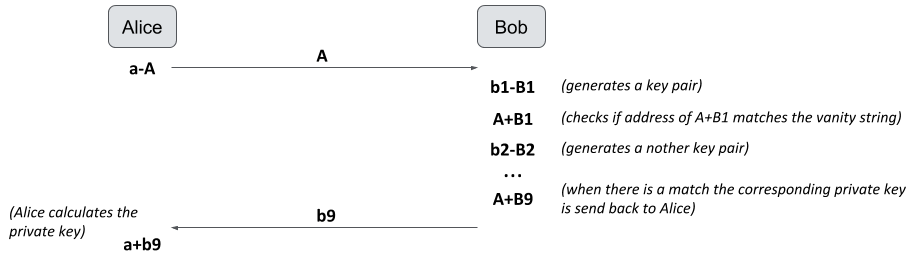
\includegraphics[scale=0.5]{images/vanity-address-pools}
\caption{Example of how a vanity address pool securely shares the private key to a user.}
\label{fig:vanity-address-pools}
\end{center}
\end{figure}

\begin{itemize}
\item First Alice creates a key pair and sends the public key \keyword{A} to Bob.
\item Bob creates a key pair and adds the new public key \keyword{B1} to Alice's key. Then uses the resulting public key to generate an address. If this address does not match the vanity string required by Alice, it repeats the process by creating another key pair, and so on. When a match is found the respective private key, e.g. \keyword{b9}, is send to Alice.
\item Now Alice, and only Alice, can construct a private key that corresponds to the vanity address by adding it to her private key. 
\end{itemize}



\section{Wallets}

A wallet is software that allows us to manage the private and public keys as well as our Bitcoin addresses. They usually have functionality to send bitcoins, check balances, create contact lists and other. Usually a key (i.e. address) is used only once. Depending on how the private keys are handled there are two types of wallets:

\begin{description}
\item[Non-deterministic] All the private keys on the wallet are just randomly generated. Several private keys are pre-generated and new keys are created if needed. If you backup your wallet and then create new keys, you will need to backup your wallet again.
\item[Deterministic] A seed is used to create a master private key, which can be used to create all other private keys (thus public keys and addresses as well). If you backup your seed you are safe no matter how many keys you use since all can be generated from the seed.
\end{description}

Nowadays, most wallets are \emph{Hierarchical Deterministic (HD)} since they offer more flexibility, easier backups and enchanced security in certain use cases. HD wallets are described in detail in \emph{Bitcoin Improvement Proposals (BIPs)} 32\footnote{https://github.com/bitcoin/bips/blob/master/bip-0032.mediawiki}, 43\footnote{https://github.com/bitcoin/bips/blob/master/bip-0043.mediawiki} and 44\footnote{https://github.com/bitcoin/bips/blob/master/bip-0044.mediawiki}. 


\section{More examples}
This section will provide more examples of how to create and use keys and addresses using the \keyword{bitcoin-utils} Python library.

\subsection*{Create a P2SH-P2WPKH address}
In this example we will create and display a P2SH address that wraps a P2WPKH script. For more details on what P2SH and P2WPKH are please refer to sections \ref{sec:p2sh} and \ref{sec:segwit} respectively.

\vspace{1em}
\begin{lstlisting}[style=Python]
>>> from bitcoinutils.setup import setup
>>> from bitcoinutils.keys import PrivateKey, P2shAddress 
>>> setup('testnet')
'testnet'
>>> native_p2wpkh = PrivateKey.from_wif('cTmyBsxMQ3vyh4J3jCKYn2A'\
...         'u7AhTKvqeYuxxkinsg6Rz3BBPrYKK').get_public_key().get_segwit_address()
>>> print("P2WPKH:", native_p2wpkh.to_string())
P2WPKH: tb1qsd4ax84vhem5hxgxus2u232nw9ylgftkz0szf2
>>> nested_p2wpkh = P2shAddress.from_script(native_p2wpkh.to_script_pub_key())
>>> print("P2SH(P2WPKH):", nested_p2wpkh.to_string())
P2SH(P2WPKH): 2N8Z5t3GyPW1hSAEJZqQ1GUkZ9ofoGhgKPf
\end{lstlisting}
\vspace{1em}


\subsection*{Sign message with private key and verify}
We can use a private key to sign a message. In asymmetric cryptography, the recipient can then use the corresponding public key to verify that the message was not tampered with.

\vspace{1em}
\begin{lstlisting}[style=Python,label={lst:sign-verify-message},caption={Use public key to sign a message and them verify},captionpos=b]
>>> from bitcoinutils.setup import setup
>>> from bitcoinutils.keys import P2pkhAddress, PrivateKey, PublicKey
>>> setup('testnet')
'testnet'
>>> priv = PrivateKey.from_wif('91h2ReUJRwJhTNd828zhc8RRVMU4krX9q3LNi4nVfiVwkMPfA9p')
>>> address = priv.get_public_key().get_address()
>>> message = "The test!"
>>> signature = priv.sign_message(message)
>>> print("The signature is:", signature)
The signature is: INzSwXNYNUkPFImslSFDzvqoib3ZdODcaBSZHvx5e4z1wc64cF1dVMZbDFtZxYBlD\\
L/dsjK2iBD5qAf7VcmSdQo=
>>> if PublicKey.verify_message(address.to_string(), signature, message):
...     print("The signature is valid!")
... else:
...     print("The signature is NOT valid!")
...
The signature is valid!
\end{lstlisting}
\vspace{1em}

\begin{note}
We verify using the address instead of the public key. In ECDSA cryptography the public key can be reconstructed given the signature and the public key hash (or address).
\end{note}


\section{Exercises}

\begin{exercise}
Describe possible outcomes of mistyping a Bitcoin address when trying to send some bitcoins.
\end{exercise}

\begin{exercise}
Use a \emph{vanity generator}, like https://github.com/samr7/vanitygen, to create some addresses.
\end{exercise}

\begin{exercise}
Use Python and the \keyword{bitcoin-utils} library to create a simple vanity generator.
\end{exercise}

\begin{exercise}
Write a function that creates a Bitcoin address given a public key. The only Python libraries that you are allowed to use are \keyword{hashlib} for the hashing algorithms and \keyword{binascii} to convert between hexadecimal and bytes.
\end{exercise}

\begin{exercise}
Create and display a P2SH address than contain a P2PK script using any random private key.
\end{exercise}


\chapter{Scripting}

\begin{summary}
This chapter goes deeper into what constitutes a transaction and how scripting is used to lock bitcoins and later unlock them to spend them. Several examples are provided on how to create transactions by calling a node’s API or programmatically.
\end{summary}

\section{Transactions}

A transaction sends bitcoins from one address to another and it consists of 1+ inputs and 1+ outputs. The inputs of a transaction consist of outputs of previous transactions. When an output is spend it can never be used again\footnote{Think of cash. If you give a 20 euro note you can never reuse it. You might be given change but it will be different notes or coins.}. All the bitcoins are transferred elsewhere (to a recipient, back to yourself as change, etc.). Outputs that are available to be spend are called \emph{Unspent Transaction Outputs (UTXOs)} and Bitcoin nodes keep track of the complete UTXO set.

\begin{note}
Each time funds are sent to an address a new output (UTXO) is created. Thus, the balance of an address depends on all the UTXOs that correspond to it. Bitcoin wallets hide UTXOs to make the whole experience friendlier but some wallets allow you to specify which UTXOs you want to spend if needed. When we create transactions programmatically we will deal primarily with UTXOs.
\end{note}

When an output (UTXO) is created we also specify the conditions under which this output can be spend. When you specify an input (the UTXO of a previous transaction) to spend from you have to prove that you satisfy the conditions set by the UTXO.

The spending conditions and the proof that authorizes transfer are not fixed. A scripting language is used to define them. When a new output is created a script is placed in the UTXO called \keyword{scriptPubKey} or more informally locking script.

When we want to spend that UTXO we create a new transaction with an input that references the UTXO that we wish to spend together with an unlocking script or more formally a \keyword{scriptSig}.

The standard transaction output types supported by the Bitcoin protocol are:

\begin{itemize}
\item P2PK (Pay to Public Key - not used anymore)
\item P2PKH (Pay to Public Key Hash)
\item P2SH (Pay to Script Hash)
\item P2WPKH (Pay to Witness Public Key Hash)
\item P2WSH (Pay to Witness Script Hash)
\item OP\_RETURN (allows for storing up to 80 bytes in an output)
\item Multisignature (legacy multisignature transactions; now P2SH/P2WSH is used instead)
\item Non-standard\footnote{Valid Non-standard transactions (containing scripts other than those defined by the standard transaction output type scripts) are rejected and not relayed by nodes. However, they can be mined if it is arranged with a miner.} (any other transaction)
\end{itemize}

The most common transaction output type offering a standard way of transferring bitcoins around is P2PKH (and P2WPKH), which is effectively ``pay to a Bitcoin address''. It is also possible, and used in the past, to pay directly to a public key with P2PK but that is not used anymore. Another very important transaction output type is P2SH (and P2WSH) which allows locking scripts of arbitrary complexity to be used.

To define a locking and unlocking script we make use of a scripting language, simply called \emph{Script}\footnote{https://en.bitcoin.it/wiki/Script}. This relatively simple language consists of several operations each of them identified by an opcode in hexadecimal. It is a simple stack-based language that uses reverse polish notation (e.g. \keyword{2 3 +}) and does not contain potentially dangerous programming constructs, like loops; it is a domain-specific language.

\subsection*{P2PKH}

Let’s examine the standard transaction of spending a Pay to Public Key Hash. The locking script (\keyword{scriptPubKey}) that secures the funds in a P2PKH address is the following:

\begin{emphbox}
\begin{verbatim}
OP_DUP OP_HASH160 <PKHash> OP_EQUALVERIFY OP_CHECKSIG
\end{verbatim}
\end{emphbox}

As we have seen in section \ref{sec:addresses} the public key hash (PKHash) can be derived from the Bitcoin address and vice versa. Thus, the above script locks the funds that have been sent in the address that corresponds to that PKHash.

To spend the funds the owner of the private key that corresponds to that address/PKHash needs to provide an unlocking script that if we prepend to the locking script the whole script will evaluate to true. An unlocking script for a P2PKH will look like this:

\begin{emphbox}
\begin{verbatim}
<Signature> <PublicKey>
\end{verbatim}
\end{emphbox}

% TODO FUTURE SECTION
Using the private key we provide an ECDSA signature of part of the transaction that we create (see future section for more details). We also provide the public key\footnote{As we have already discussed in section~\ref{sec:addresses} the public key only appears in the blockchain after we spend from an address. This is where it appears!} for additional verification.

The validation to spend a UTXO consists of running the script of \keyword{scriptSig} plus \keyword{scriptPubKey}. Both scripts are added in the stack and executed as one script.

\subsection*{Validation of P2PKH Spending}
The validation process is described in below in a step by step explanation during script execution. In each step the script element evaluated will be highlighted (left column) and the current stack (right column) will also be displayed.

%\begin{table}
\begin{center}
\begin{longtable}[H]{ |L{0.47\linewidth}|L{0.47\linewidth}| }
\hline
\multicolumn{2}{|l|}{\emph{Step 0: Execution starts. Stack is empty.}}\\
\hline
\textsf{<Signature> <PublicKey> OP\_DUP OP\_HASH160 <PKHash> OP\_EQUALVERIFY OP\_CHECKSIG} & \\
\hline
\hline
\multicolumn{2}{|l|}{\emph{Step 1: First element is evaluated. It consists of data so it goes into the stack.}} \\
\hline
\textsf{{\color{blue}<Signature>} <PublicKey> OP\_DUP OP\_HASH160 <PKHash> OP\_EQUALVERIFY OP\_CHECKSIG} & \textsf{<Signature>} \\
\hline
\hline
\multicolumn{2}{|l|}{\emph{Step 2: Second element is also data and goes into the stack.}} \\
\hline
\textsf{<Signature> {\color{blue}<PublicKey>} OP\_DUP OP\_HASH160 <PKHash> OP\_EQUALVERIFY OP\_CHECKSIG} & \textsf{<Signature> <PublicKey>} \\
\hline
\hline
\multicolumn{2}{|l|}{\emph{Step 3: Next element is an operator that duplicates the top element of the stack.}}\\
\hline
\textsf{<Signature> <PublicKey> {\color{blue}OP\_DUP} OP\_HASH160 <PKHash> OP\_EQUALVERIFY OP\_CHECKSIG} & \textsf{<Signature> <PublicKey> <PublicKey>} \\
\hline
\hline
\multicolumn{2}{|L{0.94\linewidth}|}{\emph{Step 4: Next element is an operator that calcuates the HASH160 of the top stack element. HASH160 is equivalent to RIPEMD160( SHA256( element ) ) which is what is needed to calculate the PKH from a public key.}}\\
\hline
\textsf{<Signature> <PublicKey> OP\_DUP {\color{blue}OP\_HASH160} <PKHash> OP\_EQUALVERIFY OP\_CHECKSIG} & \textsf{<Signature> <PublicKey> <PKHash>} \\
\hline
\hline
\multicolumn{2}{|L{0.94\linewidth}|}{\emph{Step 5: Next element is data and it is pushed into the stack.}}\\
\hline
\textsf{<Signature> <PublicKey> OP\_DUP OP\_HASH160 {\color{blue}<PKHash>} OP\_EQUALVERIFY OP\_CHECKSIG} & \textsf{<Signature> <PublicKey> <PKHash> <PKHash>} \\
\hline
\hline
\multicolumn{2}{|L{0.94\linewidth}|}{\emph{Step 6: Next element is an operator that checks if the top two elements of the stack are equal and fails the script if they are not. Effectively this validates that the public key provided is indeed the one that corresponds to the PKH (or address) that we are trying to spend.}}\\
\hline
\textsf{<Signature> <PublicKey> OP\_DUP OP\_HASH160 <PKHash> {\color{blue}OP\_EQUALVERIFY} OP\_CHECKSIG} & \textsf{<Signature> <PublicKey>} \\
\hline
\hline
\multicolumn{2}{|L{0.94\linewidth}|}{\emph{Step 7: Next element is an operator that expects two elements from the stack; a signature and a public key that corresponds to that signature. If the signature is valid it returns true, otherwise false.}}\\
\hline
\textsf{<Signature> <PublicKey> OP\_DUP OP\_HASH160 <PKHash> OP\_EQUALVERIFY {\color{blue}OP\_CHECKSIG}} & \textsf{OP\_TRUE} \\
\hline
\end{longtable}
%\caption{Validation steps of P2PKH}
%\label{tab:p2pkh-validation}
\end{center}
%\end{table}

Since the script finished and the only element in the stack is now \keyword{OP\_TRUE}\footnote{Or OP\_1, i.e. true. All the operators, or opcodes, and their explanations can be found at https://en.bitcoin.it/wiki/Script} the node validated ownership of the UTXO and it is allowed to be spent. Success!

To help clarify how addresses, locking scripts and UTXOs relate please see figure~\ref{fig:utxos-pkhashes-addresses}. Addresses 1Zed, 1Alice and 1Bob are short for the actual bitcoin addresses of Zed, Alice and Bob respectively. The diagram emphasises what happens when funds are sent to an address.
\vspace{1em}

\begin{figure}[H]
\begin{center}
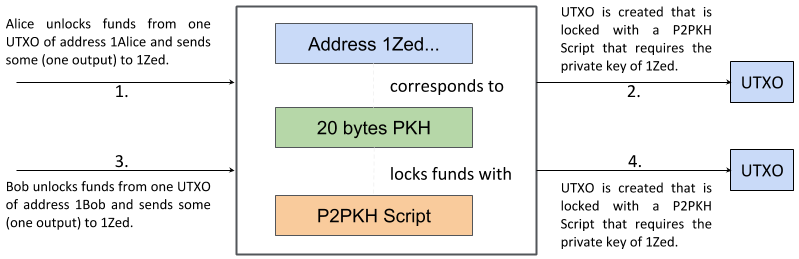
\includegraphics[scale=0.5]{images/utxos-pkhashes-addresses}
\caption{UTXOs, PKHashes and Addresses relationships.}
\label{fig:utxos-pkhashes-addresses}
\end{center}
\end{figure}

This section explained how funds residing in UTXOs are locked/unlocked and how scripts are evaluated for validation. In the next section we will go through several examples of how we can create simple transactions programmatically.



\section{Creating Transactions}

In the previous section we went through transactions, their inputs and outputs and how the funds are locked. In this post we will go through different ways of creating a simple payment transaction from the command line and then programmatically. 

\subsection*{Automatically Create a Transaction}

We can use Bitcoin's build-in command \keyword{sendtoaddress} to send bitcoins to an address.

\begin{emphbox}
\begin{lstlisting}[style=Bash]
$ ./bitcoin-cli sendtoaddress mnB6gSoVfUAPu6MhKkAfgsjPfBWmEEmFr3 0.1
18f23a2c3bea97d30e0e09376222b6888943e7dc86df43ff5dfa1ff59c10d8ec
\end{lstlisting}
\end{emphbox}

In this example we use the node to send \keyword{0.1} bitcoins to a testnet address. Notice that we do not specify any details on which UTXOs to spend from. The node wallet will decide which UTXOs it will spend and in which address the change (there is almost always change) will go; i.e. we do not have any control when sending funds this way.

\begin{note}
Notice that the result is the transaction identifier (txid) of this transaction.
\end{note}


\subsection*{Creating a Transaction using a Node}

In this example we want to select the inputs explicitly. We need to know the txids and the output indexes (vout). As an example, we can get those with:

\begin{emphbox}
\begin{lstlisting}[style=Bash]
$ ./bitcoin-cli listunspent 0
[
  {
    "txid": "b3b7464d3472a9e83da4d5c179620b71724a62eac8bc14ac4543190227183940",
    "vout": 0,
    "address": "n1jnMQCyt9DHR3BYKzdbmXWM8M5UvH9nMW",
    "account": "",
    "scriptPubKey": "76a914ddcf9faf5625d6a96790710bbcef98af9a8719e388ac",
    "amount": 1.30000000,
    "confirmations": 0,
    "spendable": true,
    "solvable": true
  }
  ...
]
\end{lstlisting}
\end{emphbox}

The above command lists all UTXOs (even those with 0 confirmations; i.e. in the mempool). Now we can create a transaction specifying the UTXO that we want to spend.


\begin{emphbox}
\begin{lstlisting}[style=Bash]
$ ./bitcoin-cli createrawtransaction '''
> [
>  {
>   "txid": "b3b7464d3472a9e83da4d5c179620b71724a62eac8bc14ac4543190227183940",
>   "vout": 0
>  }
> ]
> ''' '''
> {
>  "mqazutWCSnuYqEpLBznke2ooGimyCtwCh8": 0.2
> }'''
0100000001403918...efbe09488ac00000000
\end{lstlisting}
\end{emphbox}


The result is the serialized raw transaction in hexadecimal. Note that this is not signed yet. To see the details of the raw transaction we can use:

\begin{emphbox}
\begin{lstlisting}[style=Bash]
$ ./bitcoin-cli decoderawtransaction 0100000001403918...efbe09488ac00000000
{
  "txid": "a7b54334096108e8f69ecfa19263cfbf2f12210165ef5fc2e98ef8e4e466392e",
  "hash": "a7b54334096108e8f69ecfa19263cfbf2f12210165ef5fc2e98ef8e4e466392e",
  "size": 85,
  "vsize": 85,
  "version": 1,
  "locktime": 0,
  "vin": [
   {
    "txid": "b3b7464d3472a9e83da4d5c179620b71724a62eac8bc14ac4543190227183940",
    "vout": 0,
    "scriptSig": {
      "asm": "",
      "hex": ""
    },
    "sequence": 4294967295
   }
  ],
  "vout": [
   {
    "value": 0.20000000,
    "n": 0,
    "scriptPubKey": {
      "asm": "OP_DUP OP_HASH160 6e751b60fcb566418c6b9f68bfa51438aefbe094\\
              OP_EQUALVERIFY OP_CHECKSIG",
      "hex": "76a9146e751b60fcb566418c6b9f68bfa51438aefbe09488ac",
      "reqSigs": 1,
      "type": "pubkeyhash",
      "addresses": [
        "mqazutWCSnuYqEpLBznke2ooGimyCtwCh8"
      ]
    }
   }
  ]
}
\end{lstlisting}
\end{emphbox}

We can confirm that this is unsigned because the unlocking script or \keyword{scriptSig} is empty. We now need to sign this transaction before it becames a valid transaction.

\begin{emphbox}
\begin{lstlisting}[style=Bash]
$ ./bitcoin-cli signrawtransactionwithwallet 01000000014039...be09488ac00000000
{
  "hex": "0100000001403918270...38aefbe09488ac00000000",
  "complete": true
}
\end{lstlisting}
\end{emphbox}

Now we have the final signed raw transaction (in attribute \keyword{hex}). If we use \keyword{decoderawtransaction} now you will see the unlocking script is properly set. We can test if this is a valid transaction before sending it to the node for broadcasting with the \keyword{mempoolaccept} command. Finally, we need to send it to the node for broadcasting.

\begin{emphbox}
\begin{lstlisting}[style=Bash]
$ ./bitcoin-cli sendrawtransaction 0100000001403918270...38aefbe09488ac00000000
error code: -26, error message:, 256: absurdly-high-fee
\end{lstlisting}
\end{emphbox}

In this instance we get an error saying that the transaction has an exceptionally high fee. We have not specified any output for change so \keyword{1.1} bitcoins would be given to miners (\keyword{1.3-0.2}). Most wallets have similar protection mechanisms to help safeguard from user errors.


\subsection*{Using HTTP JSON-RPC}

JSON-RPC is a simple protocol that specifies how to communicate with remote procedure calls using JSON as the format. It can be used with several transport protocols but most typically it is used over HTTP.

A user name and password has to be provided in \keyword{bitcoin.conf}. By default only local connections are allowed, but other connections can be allowed for trusted IPs with the \keyword{rpcallowip} configuration option.

\begin{emphbox}
rpcuser=kostas

rpcpassword=too\_long\_to\_guess
\end{emphbox}

Then we could use a tool like \keyword{curl} to make the JSON-RPC request:

\begin{emphbox}
\begin{lstlisting}[style=Bash]
$ curl --user kostas --data-binary '{"jsonrpc": "1.0", "id":"curltest",  \\
"method": "getblockcount", "params": [] }' -H 'content-type: text/plain;'\\
 http://127.0.0.1:18332/
Enter host password for user 'kostas':

{
  "result": 1746817,
  "error": null,
  "id": "curltest"
}
\end{lstlisting}
\end{emphbox}

Thus, we can also send the commands seen before to construct transactions via JSON-RPC.


\subsection*{Calling Node Commands Programmatically}

A Python library that wraps Bitcoin’s API calls is \keyword{python-bitcoinrpc}. Install with \keyword{pip} and try it out.

\vspace{1em}
\begin{lstlisting}[style=Python]
from bitcoinrpc.authproxy import AuthServiceProxy, JSONRPCException

# user and pw are rpcuser and rpcpassword respectively
user = "kostas"
pw = "too_long_to_guess"     # bad practice - do not hardcode!

rpc_connection = AuthServiceProxy("http://%s:%s@127.0.0.1:18332"%(user, pw))

block_count = rpc_connection.getblockcount()
print(block_count)
\end{lstlisting}
\vspace{1em}

All API calls can be used, including the ones to create a transaction with either \keyword{sendtoaddress} or \keyword{createrawtransaction} + \keyword{signrawtransaction} + \keyword{sendrawtransaction}.



\subsection*{Creating Transactions Programmatically}

The Bitcoin node allows the creation of the basic transactions. It does not support arbitrary scripts. We can create those programmatically by explicitly specifying the locking/unlocking conditions. We will use the \keyword{python-bitcoin-utils} library that can be installed easily with \keyword{pip install bitcoin-utils} in your working python environment.

There are several examples included in the library that you can consult, like the most common transaction, a P2PKH payment\footnote{\url{https://github.com/karask/python-bitcoin-utils/blob/b31c82e7005e06db7f780688cfcd9332d479f39d/examples/p2pkh_transaction.py}} with one input and two outputs (the second output being the change).

\vspace{1em}
\begin{lstlisting}[style=Python]
# Copyright (C) 2018-2020 The python-bitcoin-utils developers
#
# This file is part of python-bitcoin-utils
#
# It is subject to the license terms in the LICENSE file found in the top-level
# directory of this distribution.
#
# No part of python-bitcoin-utils, including this file, may be copied,
# modified, propagated, or distributed except according to the terms contained
# in the LICENSE file.

from bitcoinutils.setup import setup
from bitcoinutils.utils import to_satoshis
from bitcoinutils.transactions import Transaction, TxInput, TxOutput
from bitcoinutils.keys import P2pkhAddress, PrivateKey
from bitcoinutils.script import Script

def main():
    # always remember to setup the network
    setup('testnet')

    # create transaction input from tx id of UTXO (contained 0.4 tBTC)
    txin = TxInput('fb48f4e23bf6ddf606714141ac78c3e921c8c0bebeb7c8abb2c799e9ff96ce6c', 0)

    # create transaction output using P2PKH scriptPubKey (locking script)
    addr = P2pkhAddress('n4bkvTyU1dVdzsrhWBqBw8fEMbHjJvtmJR')
    txout = TxOutput(to_satoshis(0.1), Script(['OP_DUP', 'OP_HASH160', addr.to_hash160(),
                                  'OP_EQUALVERIFY', 'OP_CHECKSIG']) )

    # create another output to get the change - remaining 0.01 is tx fees
    # note that this time we used to_script_pub_key() to create the P2PKH
    # script
    change_addr = P2pkhAddress('mmYNBho9BWQB2dSniP1NJvnPoj5EVWw89w')
    change_txout = TxOutput(to_satoshis(0.29), change_addr.to_script_pub_key())
    #change_txout = TxOutput(to_satoshis(0.29), Script(['OP_DUP', 'OP_HASH160',
    #                                     change_addr.to_hash160(),
    #                                     'OP_EQUALVERIFY', 'OP_CHECKSIG']))

    # create transaction from inputs/outputs -- default locktime is used
    tx = Transaction([txin], [txout, change_txout])

    # print raw transaction
    print("\nRaw unsigned transaction:\n" + tx.serialize())

    # use the private key corresponding to the address that contains the
    # UTXO we are trying to spend to sign the input
    sk = PrivateKey('cRvyLwCPLU88jsyj94L7iJjQX5C2f8koG4G2gevN4BeSGcEvfKe9')

    # note that we pass the scriptPubkey as one of the inputs of sign_input
    # because it is used to replace the scriptSig of the UTXO we are trying to
    # spend when creating the transaction digest
    from_addr = P2pkhAddress('myPAE9HwPeKHh8FjKwBNBaHnemApo3dw6e')
    sig = sk.sign_input( tx, 0, Script(['OP_DUP', 'OP_HASH160',
                                       from_addr.to_hash160(), 'OP_EQUALVERIFY',
                                       'OP_CHECKSIG']) )

    # get public key as hex
    pk = sk.get_public_key().to_hex()

    # set the scriptSig (unlocking script)
    txin.script_sig = Script([sig, pk])
    signed_tx = tx.serialize()

    # print raw signed transaction ready to be broadcasted
    print("\nRaw signed transaction:\n" + signed_tx)


if __name__ == "__main__":
    main()
\end{lstlisting}
\vspace{1em}

This produces the serialized raw transaction in hexadecimal. We can then use \keyword{sendrawtransaction} to send this to the Bitcoin network. Notice that \keyword{bitcoin-utils} wraps the \keyword{python-bitcoinrpc} library in a proxy object so that we can send commands to a node directly from our Python program\footnote{For an example see \url{https://github.com/karask/python-bitcoin-utils/blob/b31c82e7005e06db7f780688cfcd9332d479f39d/examples/node_proxy.py}}.



\section{Signatures}

In this section we will explain how and what needs to be signed to prove ownership of funds residing in specific addresses. 

When we create a new transaction we need to provide a signature for each UTXO that we want to spent. For a P2PKH UTXO the signature proves:

\begin{itemize}
\item that the signer is the owner of the private key
\item the proof of authorization is undeniable
\item the parts of the tx that were signed cannot be modified after it has been signed
\end{itemize}

The digital signature algorithm used is ECDSA and each signature is serialized using DER. There are different ways to sign inputs of a transaction so as to provide different commitments. For example: ``I agree to spend this input and sign it as long as no one can change the outputs I specified''. To specify these commitments, i.e. which parts of the transaction will be signed, we add a special 1 byte flag called SIGHASH at the end of the DER signature.

Each transaction input needs to be signed separately from others. Parts of the new transaction will be hashed to create a digest and the digest is what is signed and included in the unlocking script. To determine which parts are hashed the following rules are followed:

\begin{itemize}
\item all other inputs’ unlocking scripts (scriptSigs) should be empty
\item the input’s unlocking script (scriptSig), the one that we sign, should be set to the locking script (scriptPubKey) of the UTXO that we are trying to spend
\item follow additional rules according to the SIGHASH flag
\end{itemize}

The possible SIGHASH flags, values and meaning are:

\begin{description}
\item[\keyword{ALL (0x01)}] Signs all the inputs and outputs, protecting everything except the signature scripts against modification. This transaction is final and no one can modify it without invalidating this signature.
\item[\keyword{NONE (0x02)}] Signs all of the inputs but none of the outputs, allowing anyone to change where the satoshis are going. A miner will always be able to send the funds to his address. This flag is useful in combination with another inputs’ signatures using, say, \keyword{ALL} to secure the outputs. It can be used as a blank check.
\item[\keyword{SINGLE (0x03)}] Sign all the inputs and only one output, the one corresponding to this input (the output with the same output index number as this input), ensuring nobody can change your part of the transaction but allowing other signers to change their part of the transaction. The corresponding output must exist. It can be used if someone creates a transaction with some inputs that they cannot spend and specific outputs and then send to the other participants to sign (with \keyword{ALL} or \keyword{SINGLE}), if they agree.
\item[\keyword{ALL|ANYONECANPAY (0x81)}] Signs only this one input and all the outputs. It allows anyone to add or remove inputs, so anyone can contribute additional satoshis but they cannot change how many satoshis are sent not where they go. It can be used to implement kickstarter-style crowdfunding.
\item[\keyword{NONE|ANYONECANPAY (0x82)}] Signs only this one input and allows anyone to add or remove other inputs or outputs, so anyone who gets a copy of this input can spend it however they’d like. This input can be spend even in another transaction!
\item[\keyword{SINGLE|ANYONECANPAY (0x83)}] Signs this one input and its corresponding output. Allows anyone to add or remove other inputs. A potential use would be as a means to exchange colored coin\footnote{https://en.bitcoin.it/wiki/Colored\_Coins} tokens with satoshis. For example, one can create a transaction that has an input which holds 10 of their tokens and an output of 10 million satoshis to an address that they own. This transaction would be invalid since the inputs do not provide the 10 million satoshis but it can be shared with others. If someone wants to claim the 10 tokens they can add an input with at least 10 million satoshis and an output that sends the 10 tokens to them. This would complete the transaction which can then be broadcasted.
\end{description}

\begin{figure}[H]
\begin{center}
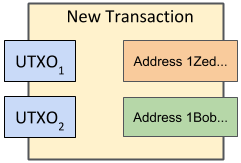
\includegraphics[scale=0.5]{images/example-transaction}
\caption{Example transaction with two inputs and two outputs.}
\label{fig:example-transaction}
\end{center}
\end{figure}

For an example of \keyword{SINGLE}, consider creating the transaction shown above. Alice needs to pay 1.5 bitcoins to Zed and they agreed with Bob that he will contribute 0.5 of that amount. Then Alice creates a transaction with two inputs, UTXO1 that she owns (with 1 BTC) and UTXO2 that Bob owns (with 1 BTC) and a single output that sends 1.5 bitcoins to Zed. She signed UTXO1 with SIGHASH \keyword{SINGLE} and sends the incomplete transaction to Bob. Bob cannot choose a UTXO other than UTXO2 since it will invalidate Alice’s signature of UTXO1. However, he is free to add other outputs so he creates an output that sends the remaining bitcoins (he agreed to pay only 0.5) to one of his addresses. He can then sign UTXO2 with SIGHASH \keyword{ALL} which will effectively finalize the transaction\footnote{No more input or output changes are allowed without invalidating this signature.}. Note that:

\begin{itemize}
\item The sequence numbers of other inputs are not included in the signature, and can be updated.
\item As already demonstrated above, with multiple inputs, each signature hash type can sign different parts of the transaction. If a 2-input transaction has one input signed with \keyword{NONE} and the other with \keyword{ALL}, the \keyword{ALL} signer can choose where to spend the funds without consulting the \keyword{NONE} signer.
\end{itemize}


\section{Pay to script hash (P2SH)}
\label{sec:p2sh}

This section explains the rationale behind Pay to Script Hash (P2SH) type of addresses and demonstrates with code.

\subsection*{Multi-signature transaction output type}
To demonstrate the advantages of P2SH we will first go through a simple use case using first the Multisignature standard transaction output type and then implement the same script with the P2SH standard transaction output type.

Consider the scenario where we accept funds in an address that is not controlled by one person. For example it is typical for companies to allow spending from corporate accounts only if, say, 2 people agree. These are called multi-signature accounts. A multi-signature account requires M-of-N signatures in order to spend the funds. An address’ locking script could enforce that. For example a 2-of-3 multi-signature locking script would look like:

\begin{emphbox}
\begin{lstlisting}[style=Pseudomath]
2 <Director's Public Key> <CFO's Public Key> <COO's Public Key> 
3 CHECKMULTISIG
\end{lstlisting}
\end{emphbox}

Indeed, this is the locking script of the multisignature standard transaction output type. If someone needs to send money (lock funds) to that output script then they need to know it! The company would need to send this script to all their customers that wish to pay them.

This is not practical since the whole script is recorded on the blockchain for every transaction and more importantly has privacy issues; the company is revealing the public keys that control the funds.

If you think about it the precise locking/unlocking script of the funds should not concern the customers at all. Only the company should know how to spend them.


\subsection*{Pay to script hash (P2SH)}
P2SH is a type of transaction output (BIP-16\footnote{https://github.com/bitcoin/bips/blob/master/bip-0016.mediawiki}) that moves the responsibility for supplying the conditions to redeem a transaction (locking script) from the sender of the funds to the redeemer (receiver).

The locking script of such a transaction is quite simple:

\begin{emphbox}
\begin{lstlisting}[style=Pseudomath]
OP_HASH160 [20-byte-hash-value] OP_EQUAL
\end{lstlisting}
\end{emphbox}

The 20-byte hash value is the hash of the redeem script:

\begin{emphbox}
\begin{lstlisting}[style=Pseudomath]
RIPEMD-160( SHA-256( 2 <Director's Public Key> <CFO's Public Key> 
<COO's Public Key> 3 CHECKMULTISIG ) )
\end{lstlisting}
\end{emphbox}

Using this hash we create a Bitcoin address (same process but instead of \keyword{OP\_HASH160(pubkey)} we use \keyword{OP\_HASH160(redeem script)}) using the version prefix of \keyword{0x05} that creates addresses that start with \keyword{3}. Consult this code for the details.

We then only need to disseminate this address to the company’s customers. The can send funds oblivious to how these funds are locked. The company knows how they are unlocked so they can prepare the appropriate unlocking script.

As an example, to spend the funds, the company can create the following script:

\begin{emphbox}
\begin{lstlisting}[style=Pseudomath]
<Director's signature> <CFO's signature> 
<2 <Director's Public Key> <CFO's Public Key> <COO's Public Key> 
 3 CHECKMULTISIG>
\end{lstlisting}
\end{emphbox}

It has two parts, the redeem script’s unlocking conditions (which in this case are two of the signatures) plus the redeem script. Notice how the redeem script is revealed only when the company spends the funds; and it only reveals the two signatures, not all three.

Validation occurs in 2 steps. First we confirm that the redeem script equals the hash in the locking script. Thus we take the second part of the unlocking script and prepend it to the unlocking script as is typically done:


\begin{emphbox}
\begin{lstlisting}[style=Pseudomath]
<2 <Director's Public Key> <CFO's Public Key> <COO's Public Key>
 3 CHECKMULTISIG>  OP_HASH160 [20-byte-hash-value] OP_EQUAL
\end{lstlisting}
\end{emphbox}

If the hashed redeem script is equal to the 20-byte hash value the above script will result \keyword{OP\_TRUE} and it validates that the correct redeem script was passed. We can now proceed in validating the actual redeem script using the first part of the unlocking script:

\begin{emphbox}
\begin{lstlisting}[style=Pseudomath]
<Director's signature> <CFO's signature> 2
<Director's Public Key> <CFO's Public Key> <COO's Public Key>
3 CHECKMULTISIG
\end{lstlisting}
\end{emphbox}

If that also results to \keyword{OP\_TRUE} then the funds can be spend.

\subsection*{Summary / Advantages}
P2SH moves the responsibility for supplying the conditions to redeem a transaction (locking script) from the sender of the funds to the redeemer (receiver).

\begin{itemize}
\item P2SH allows us to create arbitrary redeem scripts; we can thus create quite complex scripts and not be limited to the few standard transaction output types.
\item Reduces the size of the funding transactions typically resulting in saving blockchain sace.
\item Increases privacy by hiding the locking conditions.
\end{itemize}

\subsection*{Example: create a P2SH address based on a P2PK script}
As we have seen P2SH allows us to wrap arbitrary scripts hiding the script itself until it is spend. To demonstrate we will wrap a simple P2PK script and display the P2SH address that corresponds to that script.

\vspace{1em}
\begin{lstlisting}[style=Python]
from bitcoinutils.setup import setup
from bitcoinutils.keys import P2shAddress, PrivateKey
from bitcoinutils.script import Script


def main():
    # always remember to setup the network
    setup('testnet')

    #
    # This script creates a P2SH address containing a P2PK locking script
    #

    # secret key corresponding to the pubkey needed for the P2PK locking
    p2pk_sk = PrivateKey('cRvyLwCPLU88jsyj94L7iJjQX5C2f8koG4G2gevN4BeSGcEvfKe9')

    # get the public key
    p2pk_pk = p2pk_sk.get_public_key()

    # get the address (from the public key)
    p2pk_addr = p2pk_pk.get_address()

    # create the redeem script
    redeem_script = Script([p2pk_pk.to_hex(), 'OP_CHECKSIG'])

    # create a P2SH address from a redeem script
    addr = P2shAddress.from_script(redeem_script)
    print(addr.to_string())

if __name__ == "__main__":
    main()
\end{lstlisting}
\vspace{1em}

The result is address \keyword{2MvzN3FntupGqY66FuGzoK9HFXqPFyMxfVU} which can be shared to anyone that wishes to send us some funds.


\subsection*{Example: spend funds from a P2SH address}
Assuming that someone has sent funds to the P2SH address we just created let us spend it programmatically. In this example we will hardcode UTXOs for simplicity.

\vspace{1em}
\begin{lstlisting}[style=Python]
from bitcoinutils.setup import setup
from bitcoinutils.utils import to_satoshis
from bitcoinutils.transactions import Transaction, TxInput, TxOutput
from bitcoinutils.keys import P2pkhAddress, P2shAddress, PrivateKey
from bitcoinutils.script import Script

def main():
    # always remember to setup the network
    setup('testnet')

    #
    # This script spends from a P2SH address containing a P2PK script
    #

    # create transaction input from tx id of UTXO (contained 0.1 tBTC)
    txin = TxInput('7db363d5a7fabb64ccce154e906588f1936f34481223ea8c1f2c935b0a0c945b', 0)

    # secret key needed to spend P2PK that is wrapped by P2SH
    p2pk_sk = PrivateKey('cRvyLwCPLU88jsyj94L7iJjQX5C2f8koG4G2gevN4BeSGcEvfKe9')
    p2pk_pk = p2pk_sk.get_public_key().to_hex()
    # create the redeem script - needed to sign the transaction
    redeem_script = Script([p2pk_pk, 'OP_CHECKSIG'])

    to_addr = P2pkhAddress('n4bkvTyU1dVdzsrhWBqBw8fEMbHjJvtmJR')
    txout = TxOutput(to_satoshis(0.09), to_addr.to_script_pub_key() )

    # no change address - the remaining 0.01 tBTC will go to miners)

    # create transaction from inputs/outputs -- default locktime is used
    tx = Transaction([txin], [txout])

    # print raw transaction
    print("\nRaw unsigned transaction:\n" + tx.serialize())

    # use the private key corresponding to the address that contains the
    # UTXO we are trying to spend to create the signature for the txin -
    # note that the redeem script is passed to replace the scriptSig
    sig = p2pk_sk.sign_input(tx, 0, redeem_script )

    # set the scriptSig (unlocking script)
    txin.script_sig = Script([sig, redeem_script.to_hex()])
    signed_tx = tx.serialize()

    # print raw signed transaction ready to be broadcasted
    print("\nRaw signed transaction:\n" + signed_tx)
    print("\nTxId:", tx.get_txid())


if __name__ == "__main__":
    main()
\end{lstlisting}
\vspace{1em}

\begin{note}
As already mentioned, the first time we spend from the address, i.e. broadcasting this transaction, reveals the redeem script to everyone.
\end{note}



\section{Segregated Witness (SegWit)}
\label{sec:segwit}

In this section we will briefly explain what Segregated Witness is, what it changes and how scripts can be created programmatically. 

Segregated Witness is a consensus change that introduces an update on how transactions are constructed. In particular it separates (segregates) the unlocking script (witness) from the rest of the input; a transaction input does not contain an unlocking script anymore and the latter is found in another structure that goes alongside the transaction. 

To illustrate see figure~\ref{fig:tx-with-without-segwit} (i) for the original transaction that we used as an example in chapter~\ref{ch:howbitcoinworks}. We can see that the unlocking script is part of the input that we are spending. In (ii) we can see the segwit equivalent transaction where the unlocking script (\keyword{scriptSig}) is empty and it is moved outside the transaction.

\begin{figure}[H]
\begin{center}
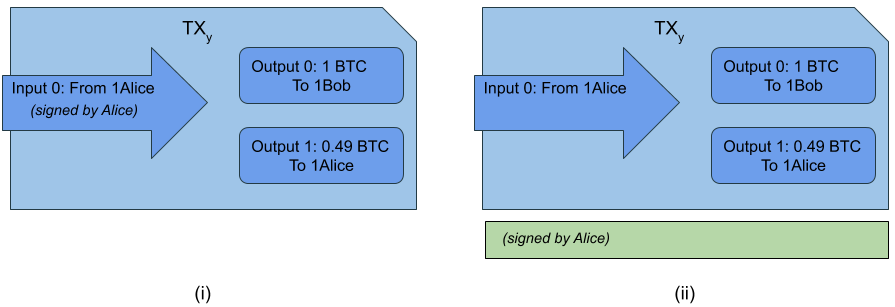
\includegraphics[scale=0.5]{images/tx-with-without-segwit}
\caption{Example transaction with (i) a non-segwit input and (ii) a segwit input.}
\label{fig:tx-with-without-segwit}
\end{center}
\end{figure}

The segwit upgrade is described in detail in BIPs\footnote{Bitcoin Improvement Proposals} 141, 143, 144 and 145 and it provides several benefits\footnote{https://bitcoincore.org/en/2016/01/26/segwit-benefits/}. We will example two of them here: \emph{transaction malleability} and \emph{effective block size increase}.

\subsection*{Transaction malleability}
Each transaction is uniquely identified by its \emph{transaction identifier} or \keyword{txid}. The \keyword{txid} is constructed by hashing\footnote{The SHA-256 hashing algorithm is applied twice.} the serialized transaction (the blue part of figure~\ref{fig:tx-with-without-segwit}).

It is possible to slightly change the unlocking script, e.g. my a miner,  so as the resulting transaction is semantically identical to the original, thus still valid. This can be accomplished, for example, by slightly changing the encoding format of the signature.

That is a problem because given how the \keyword{txid} is created even the slighest modification will change the \keyword{txid}. While the transaction is identical, i.e. funds will be moved exactly as intended, our ability to monitor this transaction is problematic given that we will be checking for confirmations in a \keyword{txid} that is not valid anymore.

With segwit inputs, however, the unlocking script (the green part of figure~\ref{fig:tx-with-without-segwit} (ii) ) is not part of the \keyword{txid} construction and thus it is impossible to modify it. A non-malleable \keyword{txid} is more reliable and allows for more advanced scripts/solutions like the lightning network.


\subsection*{Effective block size increase}
The actual block size remains the same, at 1MB. However, the unlocking scripts are now not part of the block and thus more transactions can fit into the 1MB limit.

Segwit introduces the concept of block \emph{weight} a new metric for the size of blocks. A block can have a maximum of weight of 4MBs. The non-witness part bytes of a transaction are now multiplied by 4 to get its weight while the witness part bytes are multiplied by 1, a discount of 75\%. This allows for an effective block size increase of 1.8x.

The \emph{virtual} size, or \keyword{vsize} of a transaction is the size in bytes of a transaction including the segwit discount. For non-segwit transactions\footnote{I.e. transaction with no segwit inputs.} \keyword{size} and \keyword{vsize} are identical.


\subsection*{Segwit transaction output types}
Segwit introduces two new transaction types, \emph{Pay-to-Witness-Public-Key-Hash (P2WPKH)} and \emph{Pay-to-Witness-Script-Hash (P2WSH)}, which are the segwit equivalent of P2PKH and P2SH respectively. They are sometimes called \emph{native} segwit to differentiate from \emph{nested} segwit.

The locking script (\keyword{scriptPubKey}) of these new types consists of two elements, a \keyword{version byte} and the \keyword{witness program}. The version byte introduces versioning in the witness program of the script. That is another benefit of segwit, since it allows for easy updates based on a new version.

Remember, that when signing to spend any output we need to provide the locking script, which is used to substitute the \keyword{scriptPubKey} before we calculate the transaction digest and sign it. For setwit transaction types each witness program corresponds to a predefined template script that is called \keyword{scriptCode}.

\subsubsection*{P2WPKH}
In segwit version 0, a P2WPKH witness program is just the 20-byte public key hash. The unlocking script (\keyword{scriptSig}) should be empty and the witness structure contains the unlocking script.

\begin{emphbox}
\begin{lstlisting}[style=Pseudomath]
scriptPubKey: 0 6b85f9a17492c691c1d861cc1c722ff683b27f5a
scriptSig:
witness: <signature> <pubkey>
\end{lstlisting}
\end{emphbox}

The validation is executed as follows:
\begin{enumerate}
\item The `0' in scriptPubKey specifies that the following is a version 0 witness program.
\item The length of the witness program (20-bytes) indicates that it is a P2WPKH type.
\item The witness program must consist of exactly two items.
\item The \keyword{HASH160} of the <pubkey> must match the 20-bytes witness program.
\item Finally, the signature is verified by: \keyword{<signature> <pubkey> CHECKSIG}.
\end{enumerate}

The \keyword{scriptCode} for P2WPKH is identical to P2PKH.


\subsubsection*{P2WSH}
In segwit version 0, a P2WSH witness program is just the 32-byte script hash. The unlocking script (\keyword{scriptSig}) should be empty and the witness structure contains the unlocking script as well as the \emph{witness script}\footnote{To clarify, witness script for a P2WSH is exactly what redeem script is for a P2SH.}.

\begin{emphbox}
\begin{lstlisting}[style=Pseudomath]
scriptPubKey: 0 3b892c61cc15f9a17<32 bytes>c1c722ff683b27f5a
scriptSig:
witness: 0 <signature1> <1 <pubkey1> <pubkey2> 2 CHECKMULTISIG>
\end{lstlisting}
\end{emphbox}

The validation is executed as follows:
\begin{enumerate}
\item The `0' in scriptPubKey specifies that the following is a version 0 witness program.
\item The length of the witness program (32-bytes) indicates that it is a P2WSH type.
\item The witness program must consist of the unlocking script followed by the witness script) 
\item The \keyword{SHA256} of the witness script must match the 32-bytes witness program
\item Finally, the witness script is deserialized and executed after the remaining witness stack: \keyword{0 <signature1> \emph{1 <pubkey1> <pubkey2> 2 CHECKMULTISIG}}.
\end{enumerate}

The \keyword{scriptCode} for P2WSH is the witness script.


\subsection*{Nested Segwit transaction output types}
It is possible for a non-segwit aware wallet to pay to a segwit address by embedding P2WPKH or P2WSH into a P2SH. The recipient will provide a P2SH address to the sender who can send funds as usual. The recipient can then use the redeem script which is actually the witness script to spend the funds.

\subsubsection*{P2SH(P2WPKH)}
Get the hash of the P2WPKH \keyword{scriptPubKey} and use it in P2SH as usual:

\begin{emphbox}
\begin{lstlisting}[style=Pseudomath]
HASH160 (0 6b85f9a17492c691c1d861cc1c722ff683b27f5a)
\end{lstlisting}
\end{emphbox}

And thus:

\begin{emphbox}
\begin{lstlisting}[style=Pseudomath]
scriptPubKey: <HASH160 <20-byte-script-hash> EQUAL
scriptSig: <0 <20-byte-key-hash>>
witness: <signature> <pubkey>
\end{lstlisting}
\end{emphbox}

Note that \keyword{scriptSig} contains the redeem script as a single element and without any extra unlocking data before it since those are in witness (check section~\ref{sec:p2sh} for how P2SH works). 

For validation the \keyword{scriptSig} is hashed with \keyword{HASH160} and compared to the \keyword{<20-byte-script-hash>} in \keyword{scriptPubKey}. If they are equal we can then verify the public key and signature as a native P2WPKH.


\subsubsection*{P2SH(P2WSH)}
Get the hash of the P2WSH \keyword{scriptPubKey} and use it in P2SH as usual:

\begin{emphbox}
\begin{lstlisting}[style=Pseudomath]
HASH160 (0 3b892c61cc15f9a17<32 bytes>c1c722ff683b27f5a)
\end{lstlisting}
\end{emphbox}

And thus:

\begin{emphbox}
\begin{lstlisting}[style=Pseudomath]
scriptPubKey: <HASH160 <20-byte-script-hash> EQUAL
scriptSig: <0 <32-byte-witness-script-hash>>
witness: 0 <signature1> <1 <pubkey1> <pubkey2> 2 CHECKMULTISIG>
\end{lstlisting}
\end{emphbox}

Note that \keyword{scriptSig} contains the witness script as a single element and without any extra unlocking data before it since those are in witness (check section~\ref{sec:p2sh} for how P2SH works).

For validation the \keyword{scriptSig} is hashed with \keyword{HASH160} and compared to the \keyword{<20-byte-script-hash>} in \keyword{scriptPubKey}. If they are equal we can then verify the witness script as a native P2WSH.


\subsection*{Implemented as a soft-fork}
TODO


\subsection*{Example: spend a native segwit output type}
Assuming that a P2WPKH address have some funds (UTXOs) we can use the following code to send some funds to a legacy address. As usual, we hardcode the UTXOs for simplicity.

\vspace{1em}
\begin{lstlisting}[style=Python]
from bitcoinutils.setup import setup
from bitcoinutils.utils import to_satoshis
from bitcoinutils.transactions import Transaction, TxInput, TxOutput
from bitcoinutils.keys import P2pkhAddress, PrivateKey
from bitcoinutils.script import Script

def main():
    # always remember to setup the network
    setup('testnet')

    # the key that corresponds to the P2WPKH address
    priv = PrivateKey("cVdte9ei2xsVjmZSPtyucG43YZgNkmKTqhwiUA8M4Fc3LdPJxPmZ")

    pub = priv.get_public_key()

    fromAddress = pub.get_segwit_address()
    print(fromAddress.to_string())

    # amount is needed to sign the segwit input
    fromAddressAmount = to_satoshis(0.01)

    # UTXO of fromAddress
    txid = '13d2d30eca974e8fa5da11b9608fa36905a22215e8df895e767fc903889367ff'
    vout = 0

    toAddress = P2pkhAddress('mrrKUpJnAjvQntPgz2Z4kkyr1gbtHmQv28')

    # create transaction input from tx id of UTXO
    txin = TxInput(txid, vout)

    # the script code required for signing for p2wpkh is the same as p2pkh
    script_code = Script(['OP_DUP', 'OP_HASH160', pub.to_hash160(),
                           'OP_EQUALVERIFY', 'OP_CHECKSIG'])

    # create transaction output
    txOut = TxOutput(to_satoshis(0.009), toAddress.to_script_pub_key())

    # create transaction without change output - if at least a single input is
    # segwit we need to set has_segwit=True
    tx = Transaction([txin], [txOut], has_segwit=True)

    print("\nRaw transaction:\n" + tx.serialize())

    sig = priv.sign_segwit_input(tx, 0, script_code, fromAddressAmount)
    tx.witnesses.append( Script([sig, pub.to_hex()]) )

    # print raw signed transaction ready to be broadcasted
    print("\nRaw signed transaction:\n" + tx.serialize())
    print("\nTxId:", tx.get_txid())


if __name__ == "__main__":
    main()
\end{lstlisting}
\vspace{1em}


\subsection*{Example: spend a nested segwit output type}
As described above we can also nest the new segwit address output types in a P2SH so that old non-segwit clients can send funds to new segwit-supporting clients. This example spends such a UTXO demonstrating a couple of additional details that need to be taken into consideration.

\vspace{1em}
\begin{lstlisting}[style=Python]
from bitcoinutils.setup import setup
from bitcoinutils.utils import to_satoshis
from bitcoinutils.keys import PrivateKey, P2pkhAddress, P2shAddress
from bitcoinutils.transactions import Transaction, TxInput, TxOutput
from bitcoinutils.script import Script

def main():
    # always remember to setup the network
    setup('testnet')

    # the key that corresponds to the P2WPKH address
    priv = PrivateKey('cNho8fw3bPfLKT4jPzpANTsxTsP8aTdVBD6cXksBEXt4KhBN7uVk')
    pub = priv.get_public_key()

    # the p2sh script and the corresponding address
    redeem_script = pub.get_segwit_address().to_script_pub_key()
    p2sh_addr = P2shAddress.from_script(redeem_script)

    # the UTXO of the P2SH-P2WPKH that we are trying to spend
    inp = TxInput('95c5cac558a8b47436a3306ba300c8d7af4cd1d1523d35da3874153c66d99b09', 0)

    # exact amount of UTXO we try to spent
    amount = 0.0014

    # the address to send funds to
    to_addr = P2pkhAddress('mvBGdiYC8jLumpJ142ghePYuY8kecQgeqS')

    # the output sending 0.001 -- 0.0004 goes to miners as fee -- no change
    out = TxOutput(to_satoshis(0.001), to_addr.to_script_pub_key())

    # create a tx with at least one segwit input
    tx = Transaction([inp], [out], has_segwit=True)

    # script code is the script that is evaluated for a witness program type; each
    # witness program type has a specific template for the script code
    # script code that corresponds to P2WPKH (it is the classic P2PKH)
    script_code = pub.get_address().to_script_pub_key()

    # calculate signature using the appropriate script code
    # remember to include the original amount of the UTXO
    sig = priv.sign_segwit_input(tx, 0, script_code, to_satoshis(amount))

    # script_sig is the redeem script passed as a single element
    inp.script_sig = Script([redeem_script.to_hex()])

    # finally, the unlocking script is added as a witness
    tx.witnesses.append(Script([sig, pub.to_hex()]))

    # print raw signed transaction ready to be broadcasted
    print("\nRaw signed transaction:\n" + tx.serialize())

if __name__ == "__main__":
    main()
\end{lstlisting}
\vspace{1em}


\section{Exercises}

\begin{exercise}
Write a program that spends a UTXO. The user will provide a P2PKH address as a parameter and he will then be prompted to choose between the available UTXOs of that address.
\end{exercise}

\begin{exercise}
In mainnet, how can we estimate what is an appropriate fee to include to a transaction?
\end{exercise}

\begin{exercise}
Write a scriptPubKey script that requires both a key and password to unlock.
\end{exercise}

\begin{exercise}
Create a P2SH address that corresponds to a 2-of-2 multisignature scheme. Display the address.
\end{exercise}

\begin{exercise}
Create a script that spends funds from the P2SH address created in the previous exercise.
\end{exercise}

\begin{exercise}
Write a Python function that goes through a serialized transaction and calculates what percentage of its size are the \keyword{scriptSig}s.
\end{exercise}

\begin{exercise}
Write a script that goes through a block and prints the percentage of all the \keyword{scriptSig}s relative to the size of the block.
\end{exercise}

\begin{exercise}
How can we calculate what the maximum \emph{effective} block size limit is with segwit?
\end{exercise}

\begin{exercise}
Create a P2WSH address that contains a P2PK locking script. Then display the address.
\end{exercise}

\begin{exercise}
Create a transaction that spends UTXOs from a P2WSH address that contains a P2PK locking script.
\end{exercise}

\begin{exercise}
Create a P2SH(P2WSH) address that contains a P2PK locking script. Then display the address.
\end{exercise}

\begin{exercise}
Create a transaction that spends UTXOs from a P2SH(P2WSH) address that contains a P2PK locking script.
\end{exercise}


%---------------------------------------------------------------------------
% Appendices?
%---------------------------------------------------------------------------
%\include{installnode}

\begin{lstlisting}[style=Python]
# Copyright (C) 2018-2020 The python-bitcoin-utils developers
#
# This file is part of python-bitcoin-utils
#
# It is subject to the license terms in the LICENSE file found in the top-level
# directory of this distribution.
#
# No part of python-bitcoin-utils, including this file, may be copied, modified,
# propagated, or distributed except according to the terms contained in the
# LICENSE file.

from binascii import hexlify, unhexlify
from bitcoinutils.constants import SATOSHIS_PER_BITCOIN



'''
Converts from any number type (int/float/Decimal) to satoshis (int)
'''
def to_satoshis(num):
    # we need to round because of how floats are stored insternally:
    # e.g. 0.29 * 100000000 = 28999999.999999996
    return int( round(num * SATOSHIS_PER_BITCOIN) )


'''
Counts bytes and returns them with their compact size (or varint) prepended.
Accepts bytes and returns bytes. The length should be specified in
little-endian (which is why we reverse the array bytes).

https://bitcoin.org/en/developer-reference#compactsize-unsigned-integers
'''
def prepend_compact_size(data):
    prefix = b'' 
    size = len(data)
    if size >= 0 and size <= 252:
        prefix = unhexlify(format(size, '02x').encode())
    elif size >= 253 and size <= 0xffff:
        prefix = b'\xfd' + unhexlify(format(size, '04x'))[::-1]
    elif size >= 0x10000 and size <= 0xffffffff:
        prefix = b'\xfe' + unhexlify(format(size, '08x'))[::-1]
    elif size >= 0x100000000 and size <= 0xffffffffffffffff:
        prefix = b'\xff' + unhexlify(format(size, '016x'))[::-1]
    else:
        raise ValueError("Data size not between 0 and 0xffffffffffffffff")

    return prefix + data
\end{lstlisting}




%---------------------------------------------------------------------------
% Bibliography
%---------------------------------------------------------------------------

\addcontentsline{toc}{chapter}{\textcolor{tssteelblue}{Literature}}
\printbibliography{}

%---------------------------------------------------------------------------
% Index
%---------------------------------------------------------------------------

\printindex

\end{document}
